
% TODOs:
% Get glossary working! 
% add abstract and things alike
% elaborate further on model specification
% elaborate further on word embedding! (which embedding was used?)
% elaborate further on what training data...
% elaborate further on how tokens are represented as vectors!

% Referenc ecapsule nets

\chapter{Introduction}

\section{Motivation} 

The core motivation for this thesis has been the incredible technological advance in the field of deep learning, or to be more precise: advances in neural network architectures.
\acp{ANN} are considered to be universal function
approximators \cite[chapter 4]{nielsenneural} \cite[subsection 6.4.1]{Goodfellow-et-al-2016}.
This property has enjoyed a growing potential for concrete applications and fitness for deployment throughout recent years.
A development which is also accelerated by the significant advances in parallel computing and growing accessibility of large amounts of data \cite[section 1.2]{Goodfellow-et-al-2016}.
This extraordinary development has been a key motivation for this endeavour.
The core inspiration for the ideas outlined in this paper has been a set of publications concerning novel ideas about so called \acp{CDLN} \cite{14_sparsely-gated-experts_2017}\cite{27_path-net-evolution}\cite{24_MoE-eigen2014} and their methods for hard layer routing, which seem to tackle relevant challenges in the field. 

\section{Problem}
 
This thesis seeks to answer the following main question:

\begin{center}
    \setlength{\fboxsep}{1em}
    \fbox{
       \textbf{What are the potentials and challenges of conditional neural networks?}
     }
\end{center}


However, in order to assess this question thoroughly, it will be answered through the following 4 sub-questions, addressed throughout the chapters of this thesis:

\begin{enumerate} 
  \item	How are neural network architectures commonly structured?
  \item What are possible limitations arising from these structures?
  \item What are conditional neural networks and how are they trying to tackle these limitations?
  \item What challenges are conditional neural networks facing?
\end{enumerate}
 




\section{Methods}
 
\subsection{Research}
  Prominent books about the field of deep learning establish a 
basis and serve as a source for most of the contextual claims made in this thesis.
\cite{Goodfellow-et-al-2016} \cite{nielsenneural} \cite{Patterson-Gibson-2017}
The more specific content related to concrete results is based on the 
large body of peer reviewed papers referenced throughout the chapters of this thesis.


\subsection{Search Techniques}
  
Research has been conducted based on querying search engines
like Google Scholar, Microsoft Academic and Research Gate.
In order to be able to quickly search through long blocks of texts across
a large body of research (which mostly did not end up in this thesis) carefully crafted keywords were used.
The technique was a useful tool for both
finding relevant scientific literature as well as relevant information within said literature.
It was extraordinarily useful when reading, analysing and understanding a given paper or article.
Searching for particular words on any type of literature lead to an immediate understanding of the contents at hand.
Difficult papers where information is condensed into complex paragraphs which often assume a certain context could be understood more easily by searching for unclear or unknown references in the given context.
  

\subsection{Experimentation}

Based on the theoretical groundwork layed by the discussed research in the previous chapters of this thesis, a custom neural network architecture is introduced which tries to explore a unique approach to conditional neural networks. The architecture was examined by testing it on a relatively small number of token sequences and analysing it with respect to convergence, validation loss, activity saturation and routing bias.

\clearpage
%----------------------------------------------------------------------------------------------

\section{Related Work}

The main focus of this thesis is to examine common \acf{ANN}
architectures with respect to their computation graph structure 
and compare them with approaches using conditional branching.
This thesis tries to explain the reasoning behind conditional computation
in deep learning and highlights the current and future potential of \acf{CDLN} architectures.
Large parts of it have been based on the concepts introduced in \citetitle{14_sparsely-gated-experts_2017} \cite{14_sparsely-gated-experts_2017} as well the conceptual predecessor
\citetitle{24_MoE-eigen2014} \cite{24_MoE-eigen2014} which introduced the fundamental idea of conditionally selected "\textit{experts}".
Furthermore, \citetitle{11_efficient-CDL_2017} \cite{11_efficient-CDL_2017} and \citetitle{8_CDL-4-efficient_2015} \cite{8_CDL-4-efficient_2015}
provide interesting results with respect to energy consumption
of conditional architectures.
Another interesting approach and with an even higher degree of conditional
branching is \citetitle{27_path-net-evolution} \cite{27_path-net-evolution} which
demonstrates potentials of stacked conditional layers for transfer learning with a combination of stochastic and evolutionary training.


\clearpage
%----------------------------------------------------------------------------------------------



\chapter{State of the Art}\label{chap_state-of-the-art}
 
\section{Introduction}

The field of deep learning is populated densely by a huge variety of \acp{ANN} whose use cases stretch across a wide spectrum of applications such as \acf{CV}, \acf{NLP} or general-purpose pattern recognition. 
The underlying architectures used for such tasks are too numerous to cover in one paper, however, there seem to be certain reoccurring patterns shared by many designs which may be prevalent on further inspection.
\cite[p. 12-14]{1_ANNs_2000} \cite[p. 0-1]{2_ANN-survey_2017}

Core principles of modern networks and training methods have been present since the eighties and nineties of the previous century. 
This is especially true for state-of-the-art training methods for the adjustment of weight variables in \acp{ANN}, which continue to use partial derivatives for reverse mode differentiation and error propagation, a technique famously termed back-propagation back in the 1960s and then popularized in 1986 (\citetitle{0_learning-representations-1986} \cite{0_learning-representations-1986}). 
This almost exclusively used training method is now considered the workhorse of \acp{ANN}.
\cite[p. 14-15]{1_ANNs_2000} \cite[p. ~33]{3_ANN-introduction_1993}

Although there have been interesting advances in training methods, like synthetic gradients \cite{4_synthetic-gradients_2017}, at their core, popular weight update methods seem to be mostly variations of back-propagation, relying heavily on partial derivatives and error propagation in some form. \cite[section 6.5-6.6]{Goodfellow-et-al-2016}
Therefore, this paper will not attempt to examine the current state of a potentially already established technology.
However, the following chapters will attempt to categorize and examine the architectures of popular \acp{ANN} in terms of their underlying computation graphs and structure, while also comparing them to properties of biological neural networks.

\clearpage
%----------------------------------------------------------------------------------------------


\section{The Computation Graph}

ANNs can be described via illustrations of their computation graphs, which
is especially useful when trying to differentiate them for back-propagation.
\cite[subsection 6.5.1]{Goodfellow-et-al-2016}
However, these illustrations do not adhere to a common scheme describing all architectures. 
This poses a problem when trying to comprehend, analyse, and present differences and commonalities of various \acp{ANN}.
To be able to properly examine and present multiple ANN architectures with respect to their structure, we will now proceed to define a simple illustration legend which will be used as a basis for comparing structural properties of popular \acp{ANN} in the subsequent parts of this thesis.

\begin{figure}[h]
  \centering 
    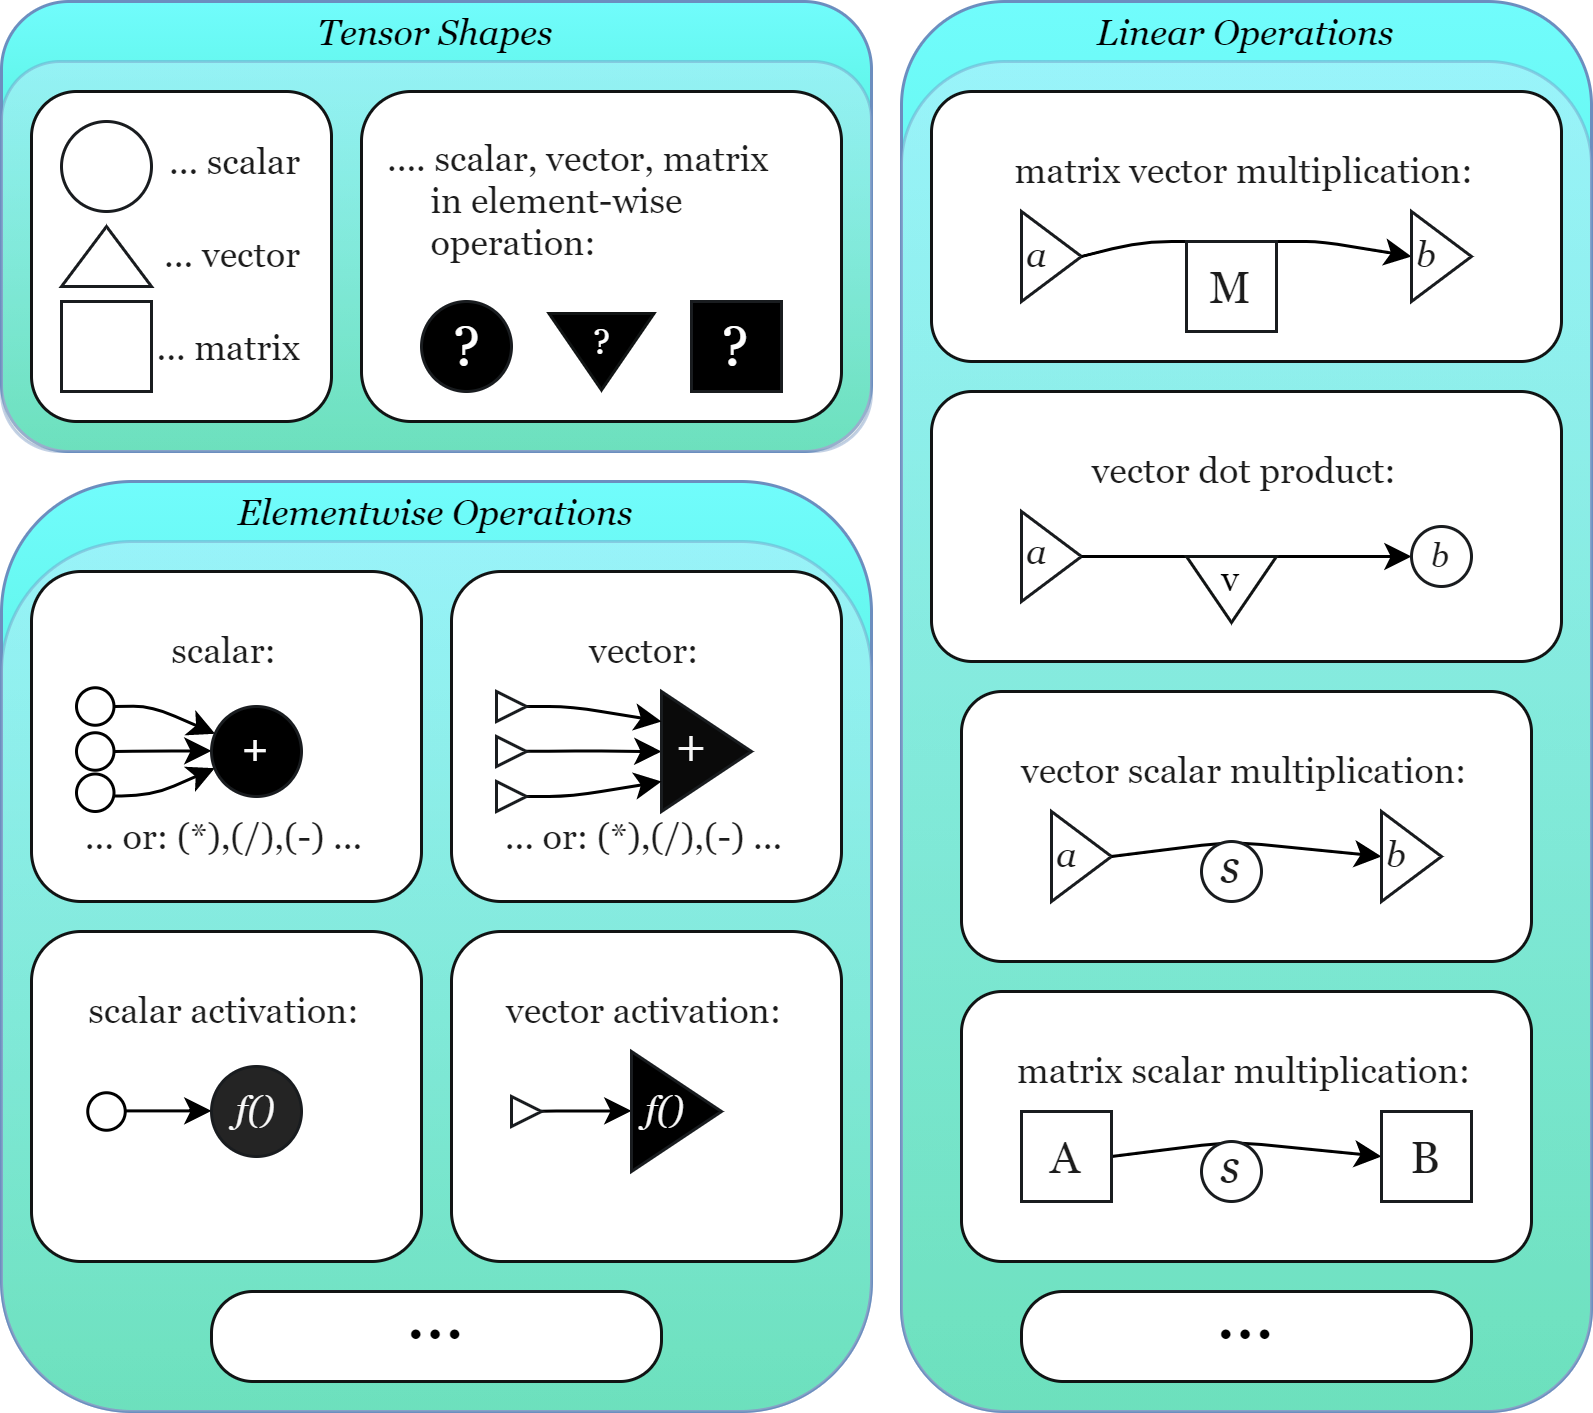
\includegraphics[width=\textwidth]{PICs/computation-graph-legend.png}
    \caption{A Computation-Graph Legend} 
\end{figure}


Similar as in other computation graphs, nodes are tensors and arrows mark their relationship as well as flow of information. There are three types of node shapes matching a corresponding tensor shape (scalar, vector, matrix) which can also be filled black to clearly identify an element-wise operation.
Linear operations on the other hand are represented by attaching the right operand (usually a weight tensor) of the operation to the edge of arrows marking state transitions. This is useful because it does not distract from the actual flow of information for a network.
 

\section{Common Neural Networks}

Extensive research about the different types of \acp{ANN} used in research and deployment, will yield a variety of architectures
which often are compositions of various design types. 
Identifying these types and assessing their popularity is challenging.
We therefore try to approximate a collection of popular designs by 
picking architectures discussed in the literature referenced by this theses.
Namely: books \cite{Goodfellow-et-al-2016}\cite{Patterson-Gibson-2017}\cite{nielsenneural}, a survey \cite{2_ANN-survey_2017} and widely shared and liked Medium articles about \acp{ANN} \cite{5_11-essential-NNs_2020}
\cite{6_10-NN-architectures_2018}, which may very well reflect the interests among the \acs{ANN} research community.
The following is the result of this approximated popularity as an unsorted list of architecture categories.
It will be examined with respect to 
a certain set of properties defined in the subsequent section.\break
 
\begin{compactitem}
  \item Simple Feed-Forward Networks \cite[chapter 6]{Goodfellow-et-al-2016}
  \item \acp{CNN} \cite[chapter 9]{Goodfellow-et-al-2016}
  \item Capsule Networks
  \item \acp{RNN} \cite[chapter 10]{Goodfellow-et-al-2016}
  \begin{enumerate}
    \item Gated Recurrent Unit Networks (GRUs)
    \item Long-Short Term Memory Networks (LSTMs)
  \end{enumerate}
  \item Residual Networks (ResNets) \cite{9_deep-res-Learning_2015}
  \item \acp{GAN}
  \item Echo State Networks (ESN) \cite[section 10.8]{Goodfellow-et-al-2016}
  \item Deconvolutional Neural Networks (DNNs)
  \item \acp{AE} \cite[chapter 14]{Goodfellow-et-al-2016}
  \begin{enumerate}
      \item \acp{VAE}
  \end{enumerate}
  \item Hopfield Neural Networks 
  \item Boltzmann Machines \cite[chapter 20]{Goodfellow-et-al-2016}
\end{compactitem}
  
\clearpage
%----------------------------------------------------------------------------------------------
 
\section{Common Properties}\label{sec_common-properties}
 
Studying these architectures gives some insight into reoccurring patterns that these networks usually have in common. 
This is especially true for the structure of the networks, more specifically the underlying structure of the computation graphs which we will discuss. 
Based on our research we will now proceed to define 3 categories / properties which are applicable to biological neural networks but only partially to popular artificial neural network architectures like those previously mentioned.

The following properties were identified and chosen based on aspects which could shine light on areas in ANN model design which potentially need improvement or further research focus. 

\clearpage
%----------------------------------------------------------------------------------------------

\subsection{Full Activity - Sparse Activity} \label{subsec_sparse-activity}

Biological neural networks are known for their sparsity, namely the observation that for a given time frame only parts of all neurons are active at high frequency, whereas large portions of the total amount of neurons stay mostly silent or fire only very infrequently.
This view is supported by data which examines the firing behavior of neurons
within the neocortical regions of the human brain. 
The following excerpt is taken from the abstract of a thorough review on this subject matter, namely \citetitle{18_experimental-evidence-of-sparsity}. 


\begin{displayquote}
\textit{
The advent of unbiased recording and imaging techniques to evaluate firing activity across neocortical neurons has revealed \textbf{substantial heterogeneity in response properties in vivo}, and that \textbf{a minority of neurons are responsible for the majority of spikes}. Despite the computational advantages to sparsely firing populations, experimental data defining the fraction of responsive neurons and the range of firing rates have not been synthesized. [...]
}
\rightline{{--- \cite{18_experimental-evidence-of-sparsity} (Abstract)}}
\end{displayquote}

It has been theorized that neurons activate selectively only for cases in which their use makes sense. This would explain away this observation of sparsity as a smart measure for energy saving \cite{19_cost-of-cortical-computation} as well as selective and local memory access, where neurons propagate their encoded information exclusively in relevant situations \cite{7_dorment-brain_2015}.
Based on this sparsity, as can be observed in nature, an \acs{ANN} architecture displaying "\textit{partial}” or “\textit{sparse}” activity will only use a subset of all containing parameters to make a single prediction. \linebreak

If we consider for example networks using the rectified-linear unit as a hidden activation function, then the produced hidden states will partially be populated by zeros for negative or zero input scalars. In theory, any linear propagation following after these states can be omitted, as they will not influence the network any further. \cite[p.1, p.8]{23_low-rank-conditional-davis2014}

\begin{wrapfigure}{R}{0.45\textwidth}
    \centering 
    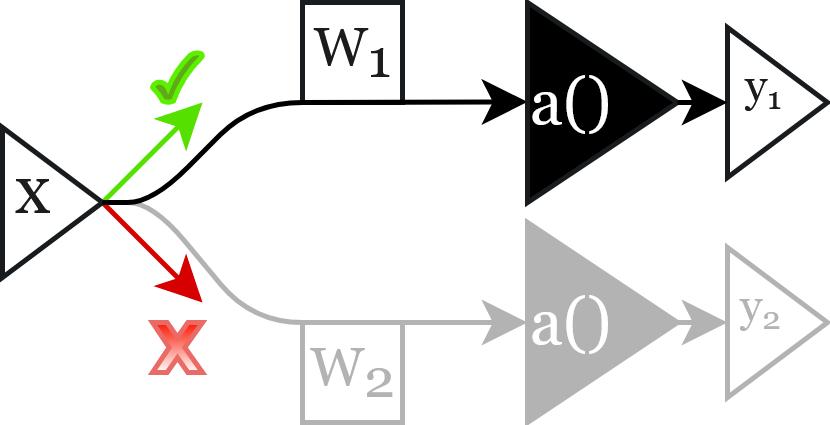
\includegraphics[width=0.40\textwidth]{PICs/sparse-activity.png}
    \caption{Sparse Activity}
\end{wrapfigure}

However, in practice, no such distinction will be made when propagating 
information through a traditional \acs{ANN}.
An exception to this would be so called “\textit{\acp{CLNN}}” which either have stacked hidden layers which are being chosen for activation selectively or simply output the results at any layer (based on certain confidence conditions) to save computational costs.
\cite[p. 1]{8_CDL-4-efficient_2015}


Conversely to biological neural networks,  \acp{ANN} usually however display “\textit{full activity}”.
This is the case if every parameter of the network is involved in forming an output given any input that is being fed into the neural network.
The vast majority of current state of the art network architectures fall under the category of “\textit{full activity}” networks. ( \acp{CNN} / DNNs, FFNNs,  \acp{RNN},  \acp{AE}, …)
 
 
 
\clearpage
%----------------------------------------------------------------------------------------------



\subsection{Feed Forward - Computation Graph Branching}\label{subsec_feed-forward}


\acp{ANN} are at their core merely differentiable computation graphs consisting of tensors and operations. The usage of tensors is especially helpful because they are an abstraction of 
scalars, vectors and matrices \cite{22_era-of-big-data-processing} \cite[section 2.1]{Goodfellow-et-al-2016}. In practice, this is implemented as n-dimensional arrays which enable the storage of large amounts of weight and activation scalars compactly on a single memory layer (typically in \acs{RAM}) for accelerated parallel execution ideally on a single compute device to avoid being bottle-necked by bandwidth.\linebreak

\begin{wrapfigure}{R}{0.45\textwidth}
  \centering 
  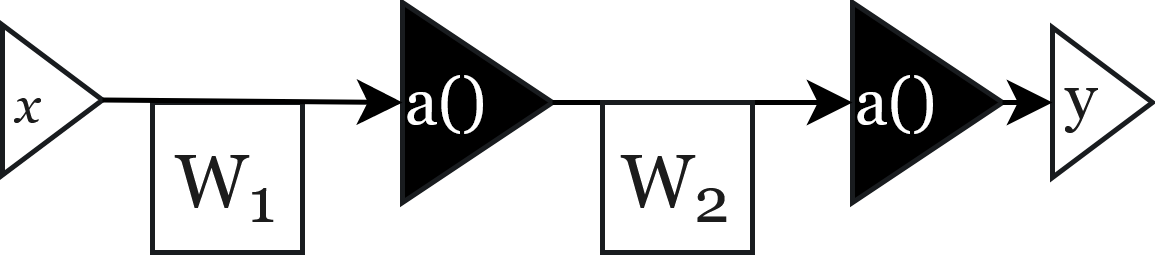
\includegraphics[width=0.40\textwidth]{PICs/simple-feed-forward.png} 
  \caption{A CG of a FFNN}
\end{wrapfigure}

When viewing a traditional feed forward neural network as a computation graph of tensors and operations then this graph structure does not contain branches \cite[chapter 6]{Goodfellow-et-al-2016}.
During execution the entire model resides in RAM and all parameters are being utilized to form a given output. \linebreak
  

However theoretically introducing branches would allow for selective / sparse activity propagation (subsection \ref{subsec_sparse-activity}) and therefore the ability to store inactive branch variables on slower memory with higher capacity until needed again.


\begin{wrapfigure}{L}{0.45\textwidth}
  \centering 
  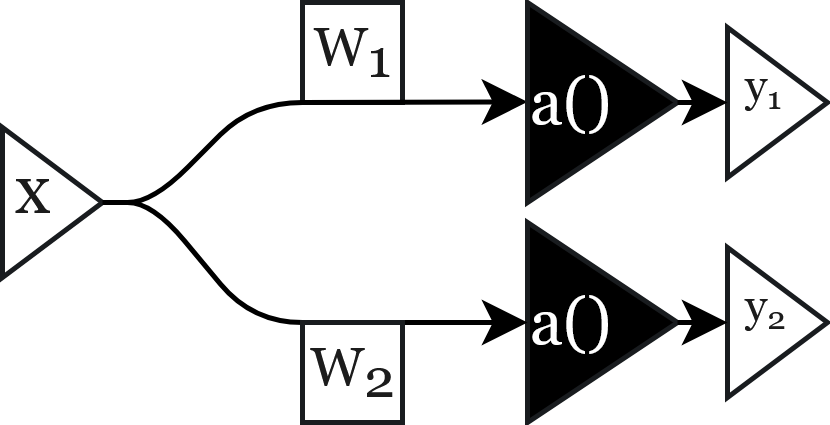
\includegraphics[width=0.40\textwidth]{PICs/branching-illustration.png}
  \caption{Branching CG}
\end{wrapfigure}
 

Based on that, a neural network architecture has so called “computation graph branches” if the flow of information goes through different (linear) tensor operations which eventually merge back together to ultimately form the final output.
Branching for different elementwise operations does not count as computation graph branching because they can easily be performed within a single activation, however two weight tensors and different elementwise activations applied to one forward pass would fall under this definition.\linebreak

\begin{wrapfigure}{R}{0.45\textwidth}
  \centering 
  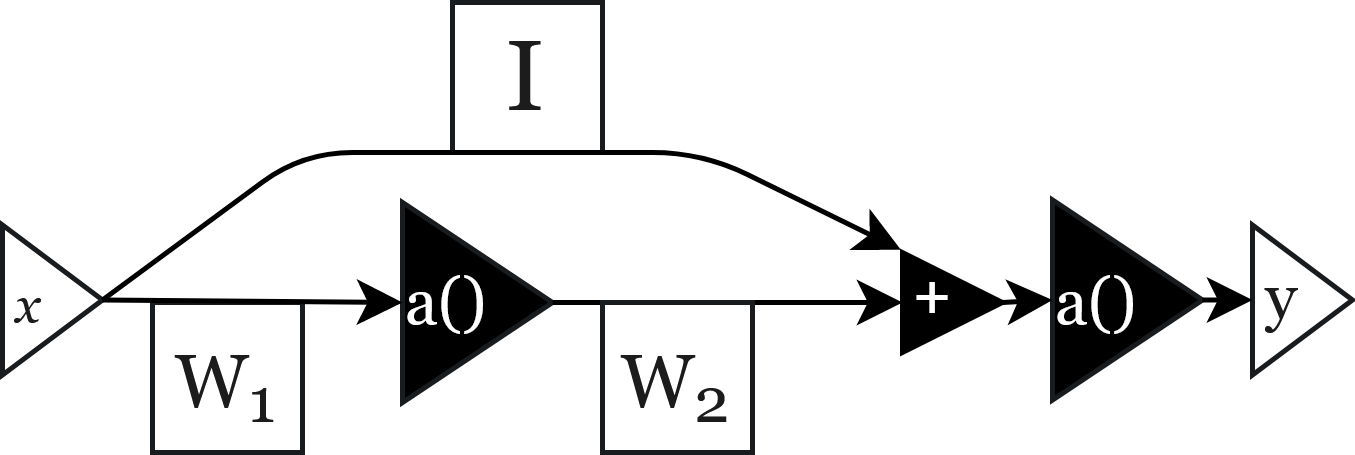
\includegraphics[width=0.40\textwidth]{PICs/residual-layer.png} 
  \caption{A residual layer}
\end{wrapfigure}

A good example of this property can be found in ResNet, in which previous layer results are being copied back into layers further down the end of the network. 
Components performing this operation are being referred to as “residual layers”.
\cite{9_deep-res-Learning_2015}
 
 
\clearpage
%----------------------------------------------------------------------------------------------




\subsection{Directed A-Cyclic - Recurrent}\label{subsec_directed-a-cyclic}

As previously mentioned, the underlying architecture of many ANNs adheres to a feed forward pipeline-like structure. In such networks information flows solely in one direction, meaning that such a neural network cannot retain information of previous forward passes. 

In essence such a design can be viewed as an acyclic directed computation graph \cite[chapter 6]{Goodfellow-et-al-2016}. Therefore, it is not only a pure method in a computational sense, but also a mathematical (total) function being both left-total as well as right-unique (for tensors). 
This is based on the fact, that traditionally ANNs consist of simple linear and non-linear operations forming a directed acyclic (computation) graph (DAG) of tensors and operations. 
\cite[p. 8-10]{10_rec-NN-Review_2015} The most obvious example of such a “pipeline” neural network architecture would be a standard feedforward neural network.\linebreak

 
\begin{wrapfigure}{R}{0.45\textwidth}
  \centering 
  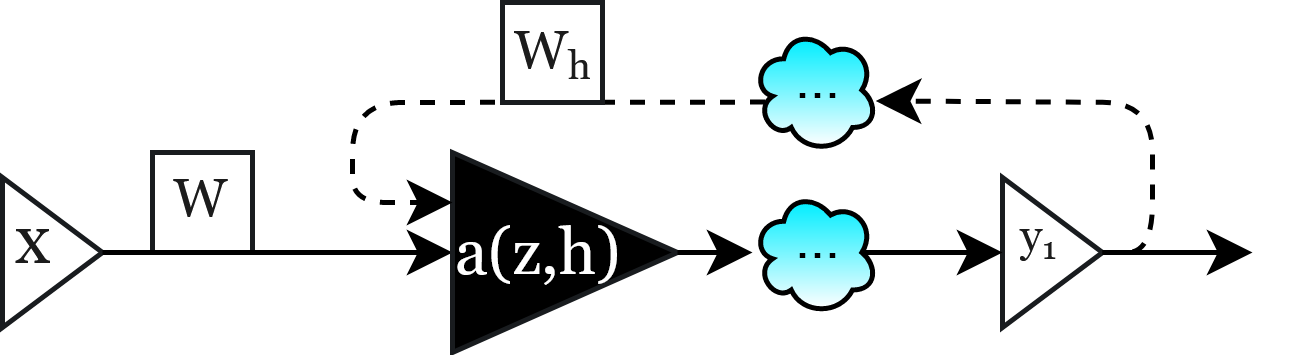
\includegraphics[width=0.40\textwidth]{PICs/cyclic-graph.png}
  \caption{A computation graph demonstrating a recurrent flow of information.}
  \label{cyclic-graph}
\end{wrapfigure}

Conversely an ANN deviating from this design would be a \acf{RNN} which would also allow for cyclic propagation of information through the computation graph.
 \cite[p. 143]{Patterson-Gibson-2017} \cite[p. 10-13]{10_rec-NN-Review_2015}
This flow of information is being illustrated by Figure \ref{cyclic-graph}. Recurrency is a key property found in biological neural networks which are notoriously cyclic
\cite{28_recurrence-in-BNN-Kietzmann_2019} \cite{29_recurrence-in-BNN-Kohitij354753}.

Therefore future ANN models aiming towards achieving \acf{AGI} surely would need to have some form of recurrent flow of information incorporated into them.
 


 
\clearpage
%----------------------------------------------------------------------------------------------


\subsection{Batch Learner - Online Learner}\label{subsec_batch-learner}

%The general inefficiency of batch training for gradient descent learning

State of the Art \acp{ANN} are most often trained on multiple samples at once. 
\cite[p.1]{30_online-deep-learning}
These sets of samples, often referred to as batches \cite[chapter 4]{LeCunBOM12}, are being fed into a given network in the form of one or more large tensors storing these stacked samples densely in RAM, which is why memory is often a determining factor for the batch size \cite[subsection 8.1.3]{Goodfellow-et-al-2016}.  
The final gradients applied
to the weight parameters of a given network
will then be the average of the gradients 
produced by the set of samples.
This approach is the reason why state of the art \acp{ANN} are generally being referred to as \textit{batch learner} \cite[p.1]{30_online-deep-learning}. \linebreak
It has several advantages:

\begin{itemize} 
  \item	
  As an average of many gradients the final gradient applied to the weights will have less
noise, which makes it a more informed step towards the global.
  \item 
  This reduced level of noise will ensure a more stable
convergence during training.
  \item
  Using batches also enables the use of \acf{SIMD} dedicated hardware like GPUs, 
  which greatly accelerates the propagation of multiple samples through the network.


\rightline{{--- \cite[chapter 4]{LeCunBOM12}}}

\end{itemize}
 

However, there seem to be trade-offs associated with this approach.
As observed by Nitish Shirish Keskar et al.
\cite{26_large-batch-keskar2017} :

\begin{displayquote}
 
\textit{The stochastic gradient descent method and its variants are algorithms of choice for many Deep Learning tasks. These methods operate in a small-batch regime wherein a fraction of the training data, usually 32--512 data points, is sampled to compute an approximation to the gradient. \textbf{It has been observed in practice that when using a larger batch there is a significant degradation in the quality of the model, as measured by its ability to generalize.} 
There have been some attempts to investigate the cause for this generalization drop in the large-batch regime, however the precise answer for this phenomenon is, hitherto unknown. In this paper, we present ample numerical evidence that supports the view that large-batch methods tend to converge to sharp minimizers of the training and testing functions -- and that sharp minima lead to poorer generalization. In contrast, small-batch methods consistently converge to flat minimizers, and our experiments support a commonly held view that this is due to the inherent noise in the gradient estimation. We also discuss several empirical strategies that help large-batch methods eliminate the generalization gap and conclude with a set of future research ideas and open questions.}
 
\rightline{{--- \cite{26_large-batch-keskar2017} (Abstract)}}

\end{displayquote}

This degradation in performance when using larger batches has lead to a more balanced approach, namely the use of so called \textit{mini-batches}, which are simply smaller
batches whose size might be adjusted during training.
\cite[chapter 4.1]{LeCunBOM12}


Not using a batch at all and merely calculating a gradient based on a single sample
is being referred to as \textit{stochastic learning}, or more generally \textit{online learning} \cite[chapter 4.1]{LeCunBOM12} \cite{30_online-deep-learning} \cite[subsection 8.1.3]{Goodfellow-et-al-2016}. 
Although this approach is faster, because less data and computational
resources are needed for the adjustment of weights,
the calculated gradient will contain much more noise.
This noise will translate to the weights of a given network when applying
the gradient, which is widely believed to be the reason why this approach
is susceptible to a phenomenon called \textit{catastrophic inference},
which is simply the observation that \acp{ANN} tend to forget what has already been learned upon introducing new information (or noise) \cite[p. 1]{20_catastrophic-inference}.
\linebreak

% TODO: Online good because real world streams of data. 
% TODO: Online good because BNNs

Finally, batch learning is an artificial learning method.
Evidently, \acp{BNN}, as can be experienced in day to day live,
receive, process and learn newly introduced information sequentially
and not in the form of batches.
 

\clearpage
%----------------------------------------------------------------------------------------------

\section{Resulting Property Table}

The properties defined under the previous section, namely
\textit{sparse/full activity} (\ref{subsec_sparse-activity}), 
\textit{feed forward/branching} (\ref{subsec_feed-forward}), 
\textit{a-cyclic/recurrent} (\ref{subsec_directed-a-cyclic}) and \textit{batch/online learning} (\ref{subsec_batch-learner}), 
either apply to a given network or they do not, 
meaning the properties are boolean in nature. Running these three properties through my list of common neural networks will yield the following truth table:


\begin{table}[h] 
\centering
 \begin{tabular}{||c | c c c c||} 
 \hline
 \acs{ANN} Type & Recurrency & Branching & Sparse Activity & Online Learner \\ [0.5ex] 
 \hline\hline
 Feed-Forward Networks & False & False & False & False \\ 
 \hline
 ResNets & False & True & False & False \\
 \hline
 RNNs (LSTM, GRU) & True & True & False & False \\  
 \hline
  CNNs & False & True & False & False \\  
\hline
  Capsule Nets & False & True & False & False \\  
 \hline
  DNNs & False & False & False & False \\  
 \hline
  GANs & False & True & False & False \\  
 \hline
  AEs & False & True & False & False \\  
 \hline
  VAEs & False & False & False & False \\  
 \hline
  Hopfield NNs & True & ~False & False & False \\  
 \hline
  Boltzmann Machine & True & ~False & False & False \\  
 \hline
\end{tabular}
\caption{State of the Art \acs{ANN} architecture property truth table}   
\end{table} 

The \acs{ANN} types evaluated in this table 
ought to represent versions as they are \textit{typically}
implemented and trained.
In practise one can build variations of these types
which deviate from this overview. 
Such variations for example will be mentioned in chapter \ref{chap_conditional-NNs}.
Any of these mentioned types could for example easily 
be trained without using batches, making them technically
online learners. 
Therefore, \textit{the table above is subject
to change and may not be true in the future}.





 
\clearpage
%----------------------------------------------------------------------------------------------


\chapter{Conditional Neural Networks}\label{chap_conditional-NNs}

\section{Introduction}

As established previously, the four discussed properties apply to popular neural networks only partially or not all, despite the fact, that said properties seem to be prevalent in biological neural networks. 

This chapter will discuss a relatively novel category of neural networks which were briefly mentioned in subsection \ref{subsec_sparse-activity}, namely "\acp{CLNN}“, which are also being referred to as “\acp{CDLN}”.
\acp{ANN} falling under this category tackle
the previously discussed challenges.  
 
Such \acp{ANN} have both branching as well as sparse activity. Therefore such architectures can be arbitrarily large without considerable increases in additional computational or memory costs \cite[p. 2]{8_CDL-4-efficient_2015} and a potential increase in execution time
for forward passes \cite{25_conditional-computation-bengio2016}.
This approach has found promising use in \acf{NLP} \cite{14_sparsely-gated-experts_2017}, \acf{RL} \cite{25_conditional-computation-bengio2016}, image recognition / classification tasks where the prediction of a very large number of classes is required
\cite{11_efficient-CDL_2017} \cite{12_dynamic-routing-in-ANNs_2017}
, transfer learning \cite{27_path-net-evolution} and online learning \cite{31_continual-learning-2020}.


\section{Gating}

To achieve both branching and sparsity of activity, conditional neural networks use sophisticated gating / routing mechanism based on which the decision, which part of the network ought to be activated next, or if any further parts ought to be activated at all, is made.

These mechanisms can come in different forms, such as continuous, binary, stochastic, random or sparse functions. 

Depending on the type they can either be differentiable and therefore trainable via backpropagation \cite{24_MoE-eigen2014} \cite{25_conditional-computation-bengio2016} \cite{14_sparsely-gated-experts_2017} or they are based on other techniques like evolutionary algorithms
\cite{27_path-net-evolution}.

\clearpage
%----------------------------------------------------------------------------------------------

\section{Challenges}

\subsection{Training}
 
As previously discussed in subsection \ref{subsec_batch-learner}, traditional \acp{ANN} are batch learners, 
meaning that during training, models are being fed with a set of samples at once. 
A method commonly referred to as \textit{batching} (\textit{full-batching}, \textit{mini-batching}) \cite[p. 32-33]{Patterson-Gibson-2017}. \\

For conditional neural networks however, it is difficult to process batches containing more than one sample. This is because two distinct samples might be routed differently through the network, which means that one would have to create batches based on common activation paths for the data set. \\
This approach has been tested in \cite[p. 5]{14_sparsely-gated-experts_2017} and \cite{24_MoE-eigen2014},
where input samples were batched after running them through the gating mechanism, which in these cases is a single feed forward \acs{ANN} at the beginning of the network. 
This gating network routes
activity to a number of sub-networks referred to as \textit{experts}. 
However, depending on the gating mechanism and the degree of conditional branching, this approach might not be feasible, in which case the training can only be done by applying the training samples sequentially. \\

This severely compromises training efficiency, because the computation becomes far less parallelizable, which in many cases renders available \acs{SIMD} accelerator hardware effectively unusable. 
Besides graphical workloads, GPUs for example are highly optimized devices for parallel arithmetic types of workloads, however their performance drops drastically when attempting to introduce conditional branching as in conditional neural networks \cite[p. 2]{14_sparsely-gated-experts_2017}. \\

The previously mentioned papers \cite{14_sparsely-gated-experts_2017} and \cite{24_MoE-eigen2014} could still batch samples because the
network architecture consists of a single conditional layer only.
The architecture described in \citetitle{27_path-net-evolution} however
consists of stacked conditional layers with their own gating mechanism.
Every sample sent into this architecture might be routed differently
through the conditional layers having a unique activity path.
Contrary to the approaches taken in \cite{14_sparsely-gated-experts_2017} and \cite{24_MoE-eigen2014}, which used back-propagation as training method, 
the conditional paths in \textit{path-net} were trained using an evolutionary algorithm \cite[p. 1]{27_path-net-evolution}.

\clearpage
%----------------------------------------------------------------------------------------------


\subsection{Routing Bias} \label{subsec_routing-bias}

Another challenge for \acp{CDLN} has been the emergence of routing bias during training, where the gating mechanism will converge towards a state in which the same few sub-networks will always be chosen. This problem has been observed in
\cite{24_MoE-eigen2014} as well as in more recent work
\cite{14_sparsely-gated-experts_2017}. \\

This routing imbalance is self-reinforcing, because a choice favoured by
the gating mechanism will lead to that conditional path being trained more
thoroughly, which then will subsequently lead to it being chosen even more favorably, as it simply yields better results \cite[p. 5]{14_sparsely-gated-experts_2017}\cite[p. 2]{24_MoE-eigen2014}. \\ 

In order to mitigate this emergent bias the researchers in \cite{24_MoE-eigen2014} and
\cite{14_sparsely-gated-experts_2017} 
introduced soft and hard constraints to the gating mechanism
as well as a modified loss function which ensures that choices will
adhere to a global balance. As reported in \cite{14_sparsely-gated-experts_2017}, this 
technique forces the gating network to converge towards a state in which individual
\textit{expert layers} are chosen evenly.


\clearpage
%----------------------------------------------------------------------------------------------

\section{Potential}

\subsection{Efficiency}

Due to the fact that conditional neural networks only require a subset of their total number of parameters to produce an output, they tend to also require less computational resources and therefore display higher performance results than implementations of traditional ANN architectures.
The following results (P. Panda et al., 2015)\cite[p. 12]{8_CDL-4-efficient_2015} show the performance of conditional networks in terms of energy efficiency (computational cost) 
as well as predictive performance (accuracy).


\begin{wrapfigure}{L}{0.45\textwidth}
  \centering 
  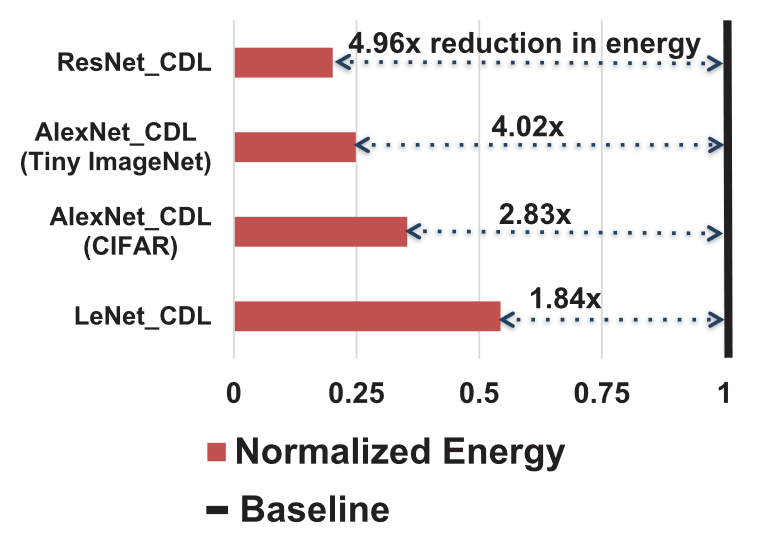
\includegraphics[width=0.40\textwidth]{PICs/CDL-energy-efficiency.png}
  \caption{Proportional Energy Efficiency comparison between \acs{CDL} and Baseline implementations.}
\end{wrapfigure}

The measurements displayed on the left are based on comparing popular neural network architectures to \acs{CDL} versions of themselves. The researchers turned these existing architectures into conditional based versions and measured their proportional energy consumption compared to their default (baseline) implementations.
The most impressive \acs{CDL} implementation, namely a version of ResNet, displayed a reduction in energy consumption by a factor of almost 5, meaning that on average the baseline implementation consumed almost 5 times more computational cost and therefore also 5 times more energy when executed. \linebreak


\begin{wrapfigure}{R}{0.45\textwidth}
  \centering 
  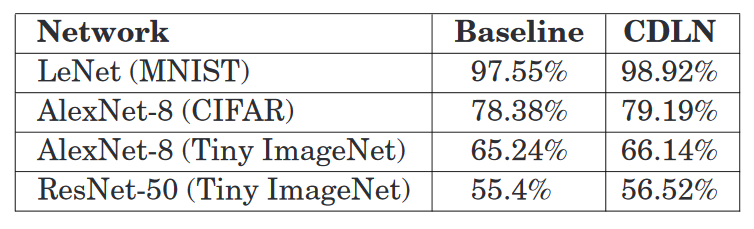
\includegraphics[width=0.40\textwidth]{PICs/accuracy-comparison-between-CDL-and-vanilla-ANNs.png}
  \caption{Accuracy of \acs{CDL} Compared to Baseline.}
  \label{accuracy-of-CDLNs}
\end{wrapfigure}

However energy efficiency alone is not relevant if the architecture does not perform well in terms of predictive performance. 
Therefore the researchers also measured 
model accuracy for both \acs{CDL} as well as baseline implementations.
These results were also promising as the accuracy of the tested models was not compromised.
 


\subsection{Robust Online Learning}

As previously mentioned in subsection \ref{subsec_batch-learner}, \acp{ANN} are known to be susceptible to a phenomenon called \textit{Catastrophic Inference}, also referred to as \textit{Catastrophic Forgetting}, which is especially true for \textit{stochastic learning} / \textit{online learning}.
This phenomenon is simply the observation that \acp{ANN} tend to forget what has already been learned upon introducing new information.
It arises due to the fact that when updating a given \acs{ANN} the parameters will be adjusted so that the model accommodates the training data introduced in the most recent epoch \cite[p. 1]{20_catastrophic-inference}.

For this reason and those previously and more thoroughly discussed in subsection \ref{subsec_batch-learner}, state of the art \acp{ANN} are being trained using batches of samples instead of single samples. \linebreak

As established in chapter \ref{chap_conditional-NNs}, executing a conditional neural network requires only a specialized subset of the total number of parameters.
Therefore, when back-propagating the error for a single training sample only this subset of parameters will be updated. Conversely, the unused parts of the network will simply stay constant. 

This inherent property of \acp{CDLN} makes them more resilient to catastrophic inference \cite[p. 1]{21_conditional-channel-gated-network}.
In theory this should make them more suitable
for being \textit{stochastic/online learner} than 
traditional \acp{ANN}.
This theoretical reasoning is also supported by the results in \cite{31_continual-learning-2020} which
demonstrate that the selectively used sub-networks referred to as \textit{experts} can mitigate the
emergence of catastrophic inference.
 
 
\subsection{Transfer Learning}

\acf{TL} is a method in which a trained model
is being incorporated into another model either fully or only
by using parts of it.

\acs{TL} has been successfully applied to \acs{CDLN}.
Promising results for this can be found in \citetitle{27_path-net-evolution} \cite{27_path-net-evolution}.

The stacked layers of the architecture described in this paper consist
of multiple sub-networks which can be activated conditionally.
By fixing certain conditional paths and transferring them 
into a new model it has been shown that this new model would 
learn significantly faster \cite[chapter 3]{27_path-net-evolution}.


\clearpage
%----------------------------------------------------------------------------------------------

\chapter{Neural Activity Routing Unit}
This chapter is dedicated to a potentially novel conditional neural network architecture which seeks to
improve upon the gating and routing mechanism of current state of the art Conditional ANN architectures. 

What follows in this chapter has been heavily inspired by

\begin{itemize} 
    \item	 \textit{"The  Sparsely-Gated  Mixture-of-Experts  Layer"} \cite{14_sparsely-gated-experts_2017} 
    \item  \textit{\citetitle{24_MoE-eigen2014}} \cite{24_MoE-eigen2014}
    \item \textit{\citetitle{27_path-net-evolution}}   \cite{27_path-net-evolution}
  
    \item \textit{\citetitle{11_efficient-CDL_2017}} \cite{11_efficient-CDL_2017}
    
    \item \textit{\citetitle{8_CDL-4-efficient_2015}} \cite{8_CDL-4-efficient_2015}
        
    \item \textit{\citetitle{12_dynamic-routing-in-ANNs_2017}} \cite{12_dynamic-routing-in-ANNs_2017}
    
    \item \textit{\citetitle{15_dynamic-routing-between-capsules_2017}} \cite{15_dynamic-routing-between-capsules_2017}  
    
\end{itemize}

The subsequent subsection will first explain 
the structure of this potentially novel 
unit architecture after which a 
custom model designed using this unit 
will be put to test.

\clearpage
%----------------------------------------------------------------------------------------------

 
A \acf{NARU} consists of two fundamental components, namely: 
 

\begin{enumerate} 
  \item \textbf{Bundles} \linebreak
  Simple sub-nets similar to the so called \textit{expert} networks
  described in \cite{14_sparsely-gated-experts_2017} and \cite{24_MoE-eigen2014} or the described \textit{modules} in \cite{27_path-net-evolution}, which 
  can either be active or dormant during a specific time step.
  
  \item \textbf{Connections} \linebreak
  Gated recurrent connections between bundles, which
  produce their inputs. 
  
\end{enumerate}
 


\begin{figure}[h]
  \centering 
    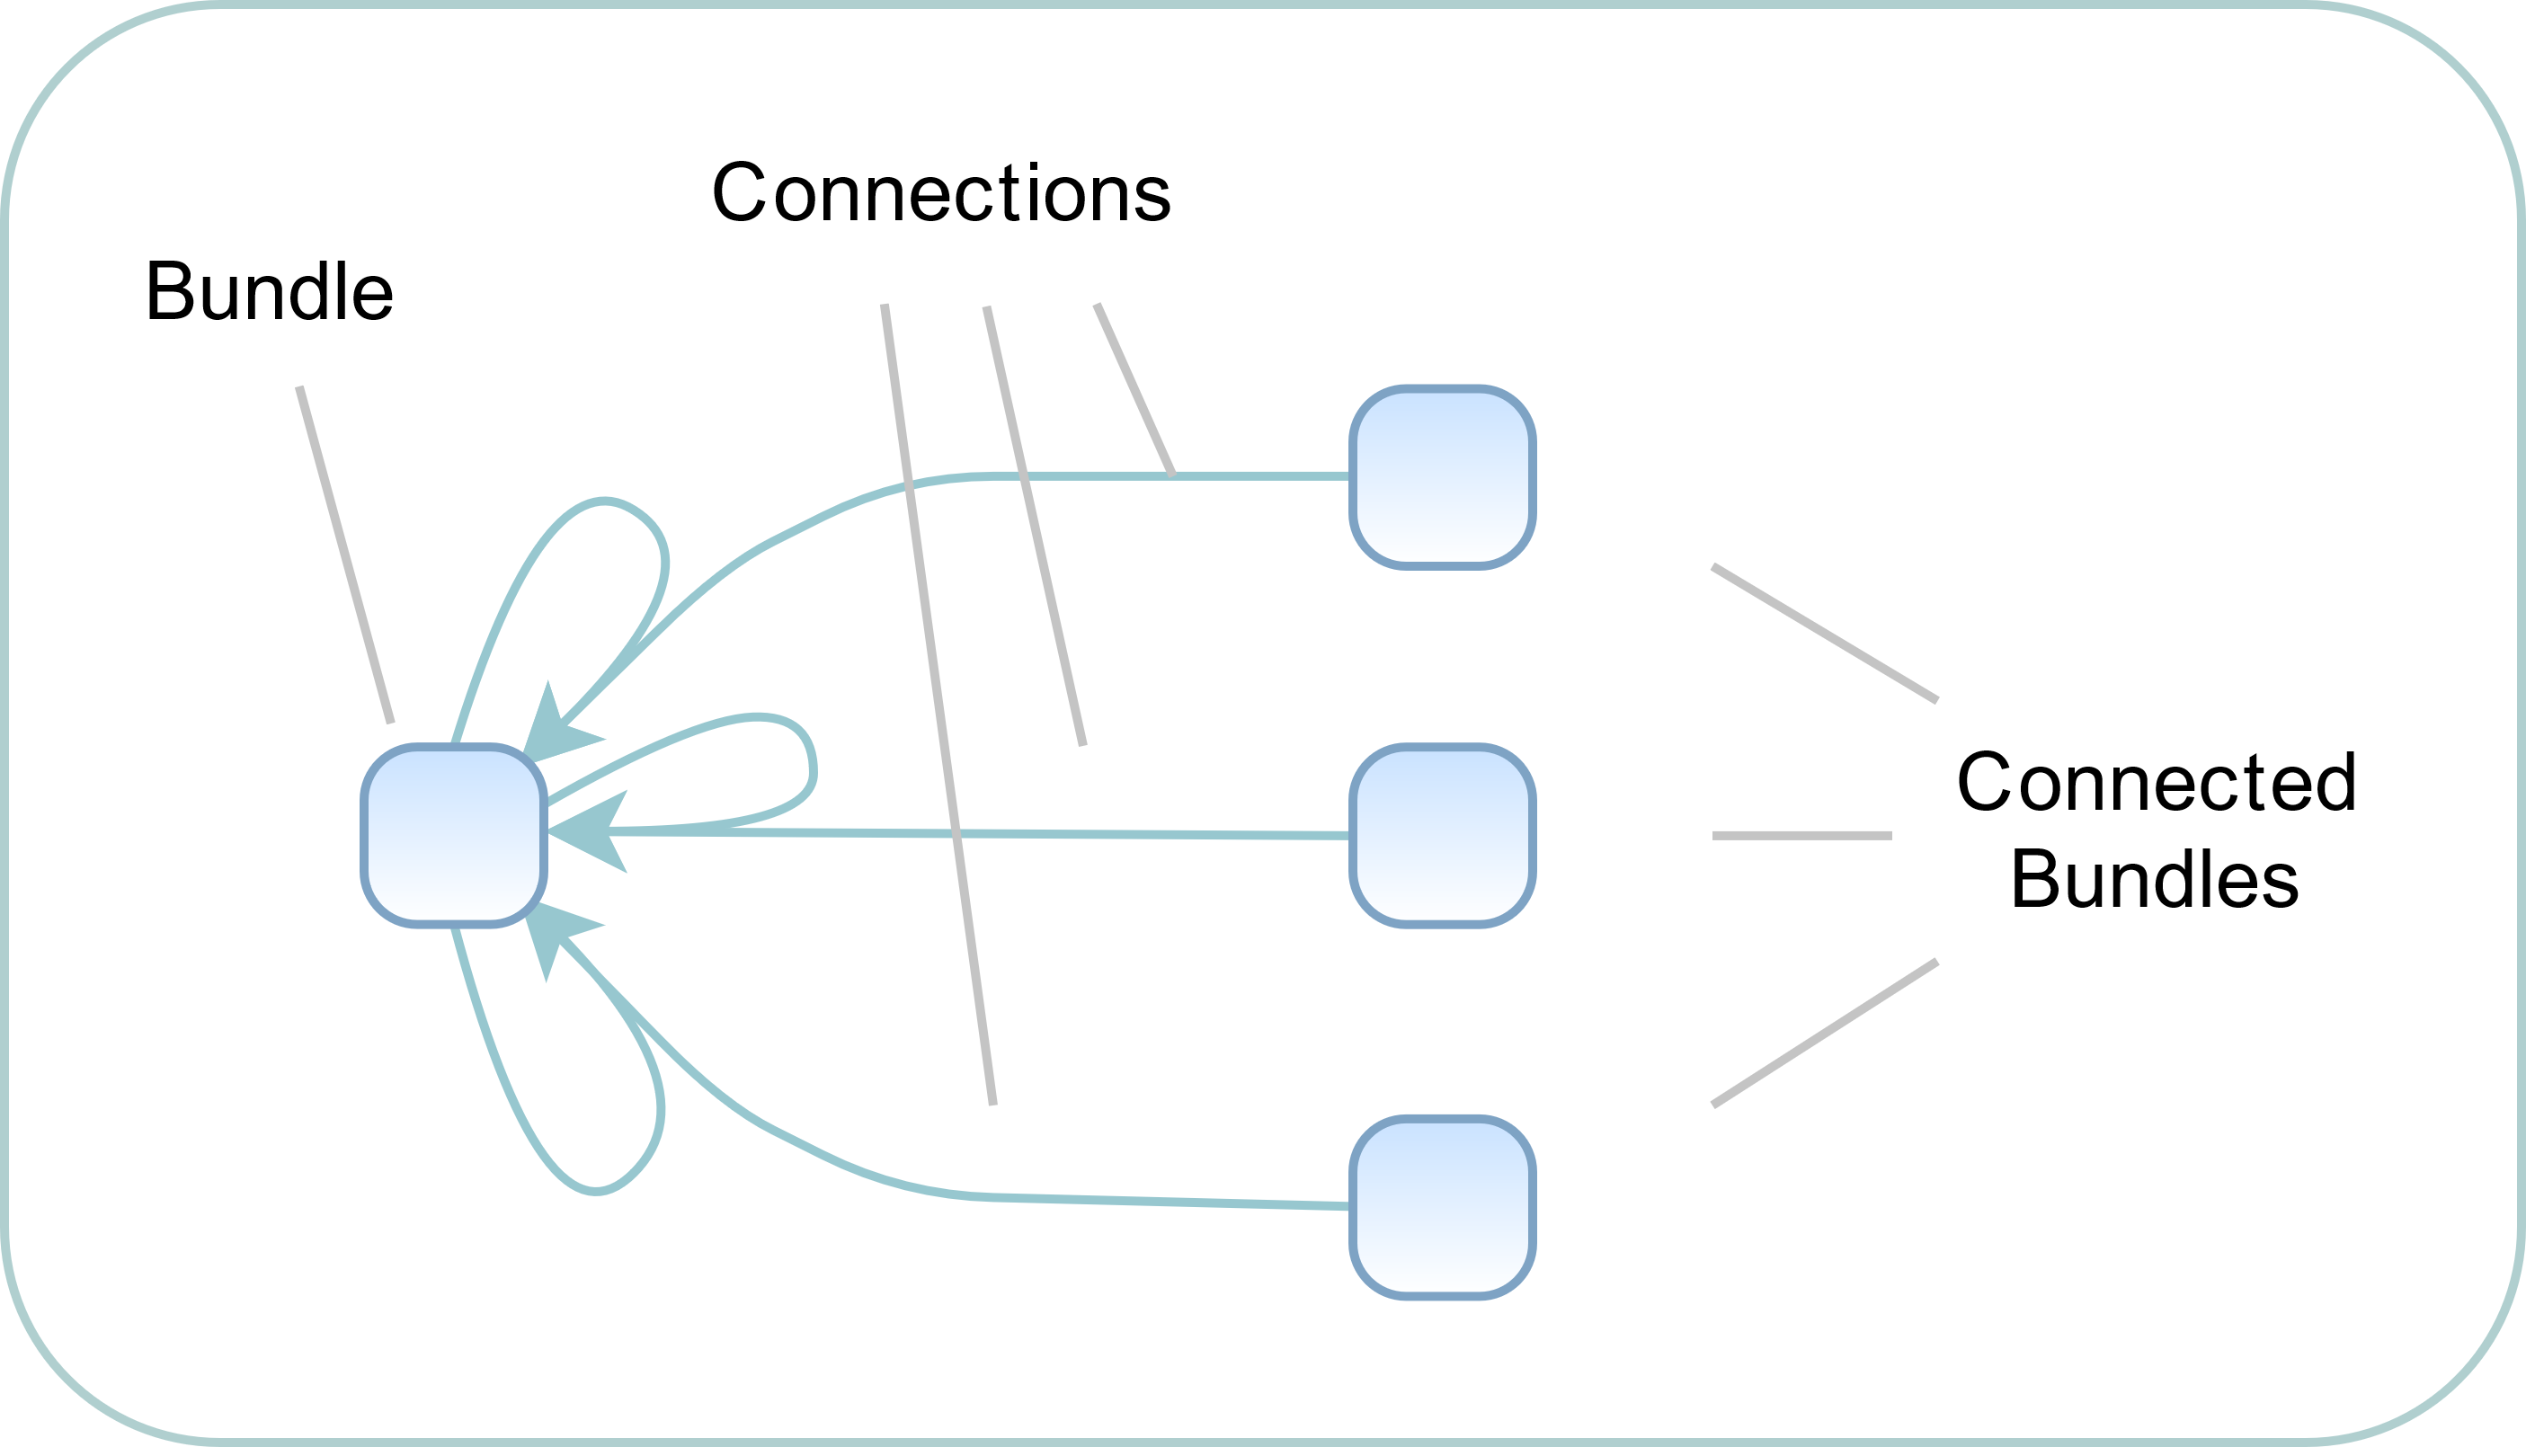
\includegraphics[width=\textwidth]{PICs/NARU/very-simple-naru.png}
    \caption{A \acf{NARU}}
    \label{very-simple-naru-illustration}
\end{figure}

A single neural activity routing unit consists of one bundle having an arbitrary number of connections whose outputs produce the input for said bundle.


\clearpage
%----------------------------------------------------------------------------------------------


\section{Connections}\label{sec_connection}

The following illustration describes the forward pass for a single connection
in terms of its computations graph. 

 
\begin{figure}[h]
  \centering 
    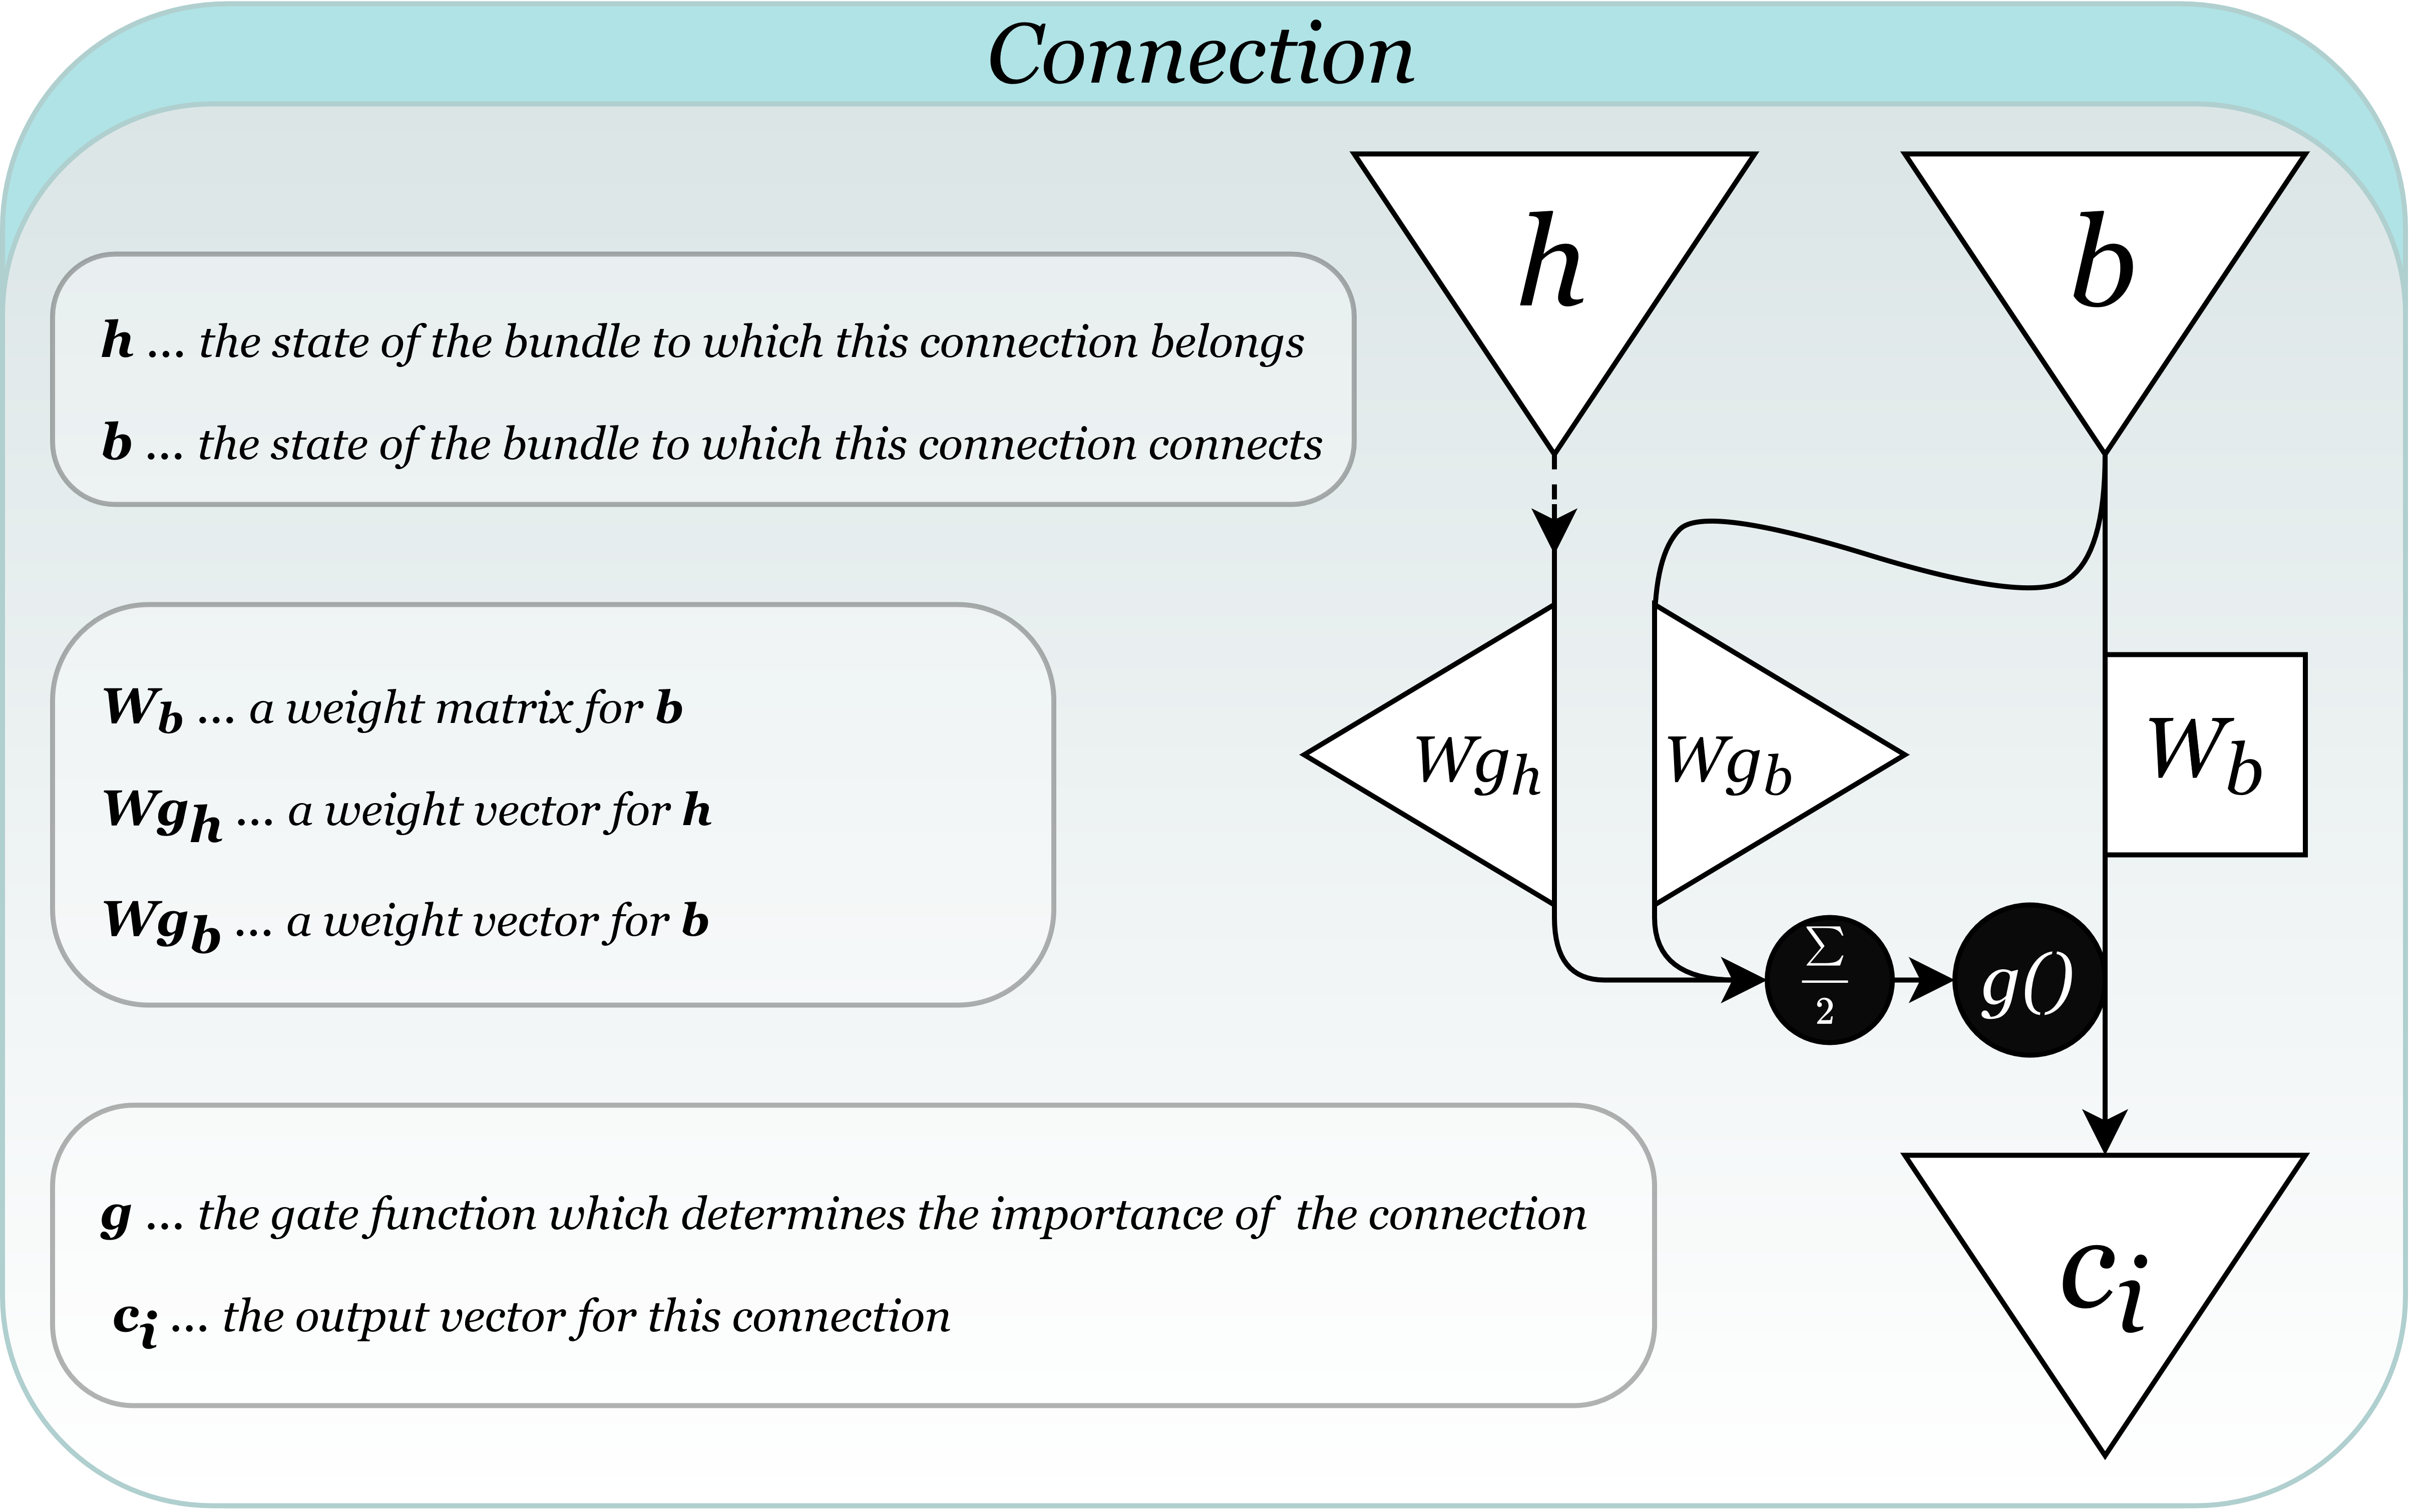
\includegraphics[width=\textwidth]{PICs/NARU/naru-connection.png}
    \caption{The Computation Graph of a Connection}
    \label{naru-Connection}
\end{figure}

A single connection receives two inputs, the state \textbf{\textit{b}} of the bundle to which it connects as well as the state \textbf{\textit{h}} of the bundle to which it belongs (time invariant).
In essence a connection is a dense feed forward pass
which is also gated. 
The vector \textbf{\textit{z}} is the result of the
weighted matrix multiplication with \textbf{\textit{b}}:


\begin{align}
z = b \cdot W_b
\end{align}

This vector will then simply be multiplied by the 
scalar value \textbf{\textit{g}}, producing
the final output of a connection, namely: \textbf{\textit{ci}}, where \textbf{\textit{i}} is the index of the current connection among all connections belonging to the current bundle.

\begin{align}
c_i = z * g
\end{align}

The calculation of the gate involves both \textbf{\textit{b}}, as well as \textbf{\textit{h}}.
The dot product of both vectors with their corresponding weight vectors \textbf{\textit{Wgb}}
and \textbf{\textit{Wgh}} produces two scalar
values whose average will be sent through a gating
function to form the final gating value.
 
\begin{align}\label{eq_gate}
    g = sig( \frac{h \cdot W_{g_h} + b \cdot W_{g_b}}{2} )
\end{align}

The full forward pass for a connection is
being described by the following expression:

\begin{align}\label{eq_full-connection-feed-forward}
c_i = (b \cdot W_b) * 
sig( \frac{h \cdot W_{g_h} + r \cdot W_{g_b}}{2} )
\end{align}
 
The results explored in this thesis are based on the implementation as described by equation \ref{eq_full-connection-feed-forward}.
However for future variations one might consider increasing the complexity of
connections to improve the performance of the network (especially with respect to the ability to routing as well as better attention).
Producing the input vector \textit{\textbf{z}} as well as its gating scalar \textit{\textbf{g}} could involve the use of more complex feed forward passes having 2 or more layers.


\clearpage
%----------------------------------------------------------------------------------------------

\section{Bundles}
 
The connection vectors \textbf{\textit{ci}} produced by the connections to other \acs{NARU} bundles will serve as inputs to a current bundle.
These vectors will be summed and divided by the total number of vectors to form a single input vector to the current bundle. A regular non-linear activation function will then be applied to 
this single input vector to form the final output of a bundle. 
Conceptually this bundle sub-network can be any feed-forward neural network, however for simplicity the reference implementation tested in this thesis does not involve more than one feed forward layer. 
 

\begin{figure}[h]
    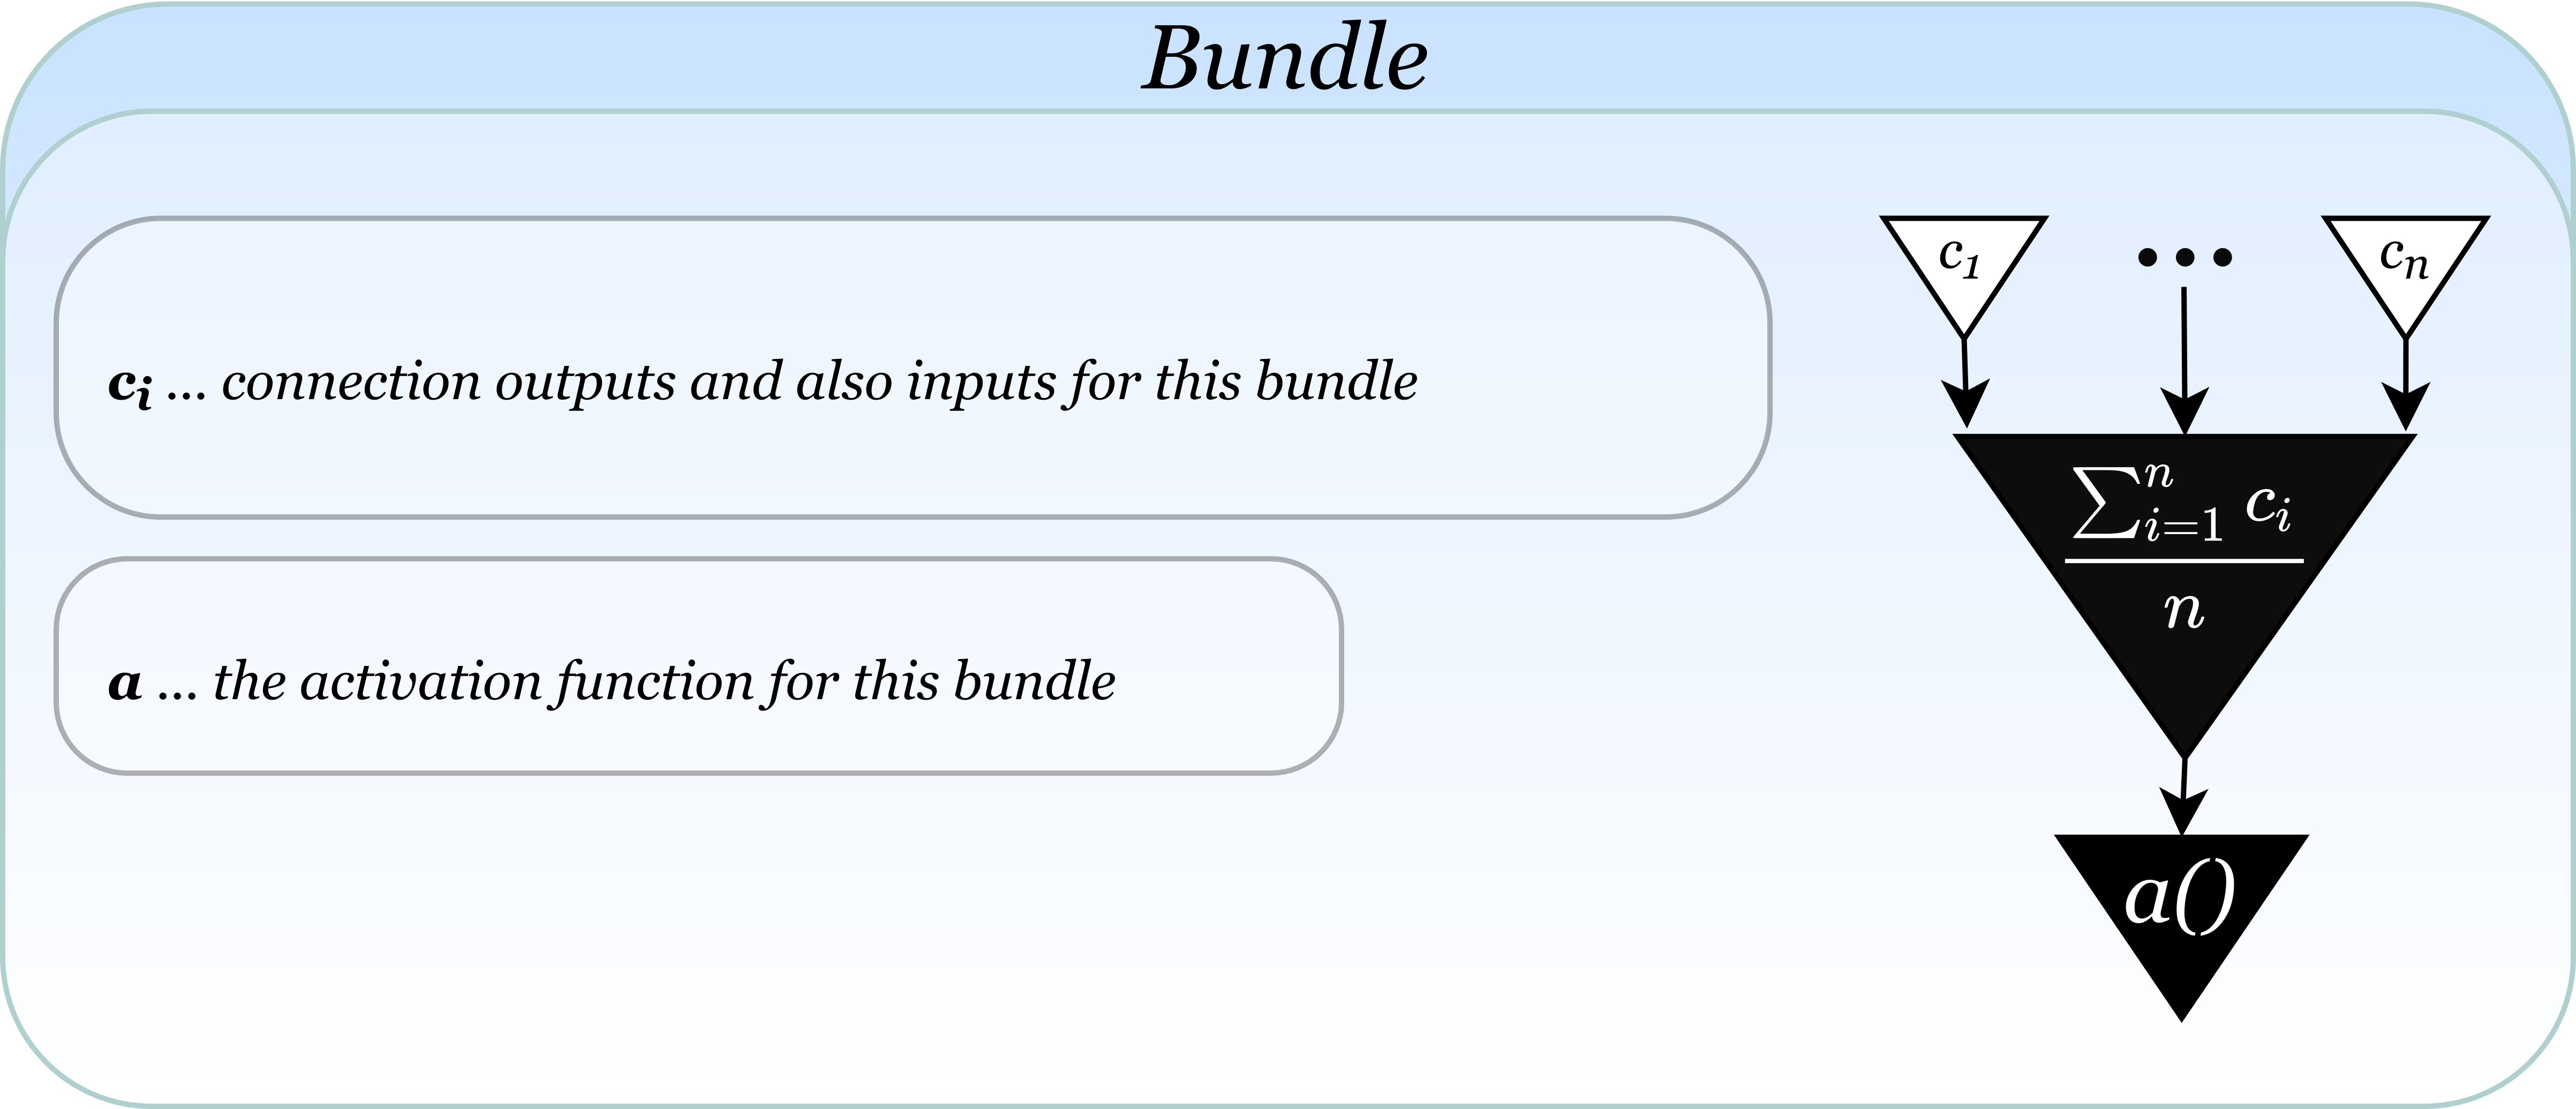
\includegraphics[width=\textwidth]{PICs/NARU/naru-bundle.png}
    \caption{The Computation Graph of a Bundle.}
    \label{computation-graph-of-a-bundle}
\end{figure}

The computation graph illustrated above can also be described by the following expression:
\begin{align}\label{eq_bundle-activation}
 b = a( \frac{\sum_{i=1}^{n} c_i}{n} ) 
\end{align}

The activation function \textit{\textbf{a}} will form the output vector \textit{\textbf{b}} which is also the final state of a bundle for a given time step \textit{\textbf{t}}. 
As referenced in section \ref{sec_connection}, in the context of a given connection, this bundle state can be any of the two variables \textit{\textbf{h}} and \textit{\textbf{b}}. However \textit{\textbf{h}} represents the previous bundle state of the current \acf{NARU} whereas \textit{\textbf{b}} will allways be the bundle state of the unit to which the current connection connects.

 \clearpage
%----------------------------------------------------------------------------------------------


\section{Routing}\label{sec_naru-routing}


\begin{wrapfigure}{R}{0.45\textwidth}
    \centering 
    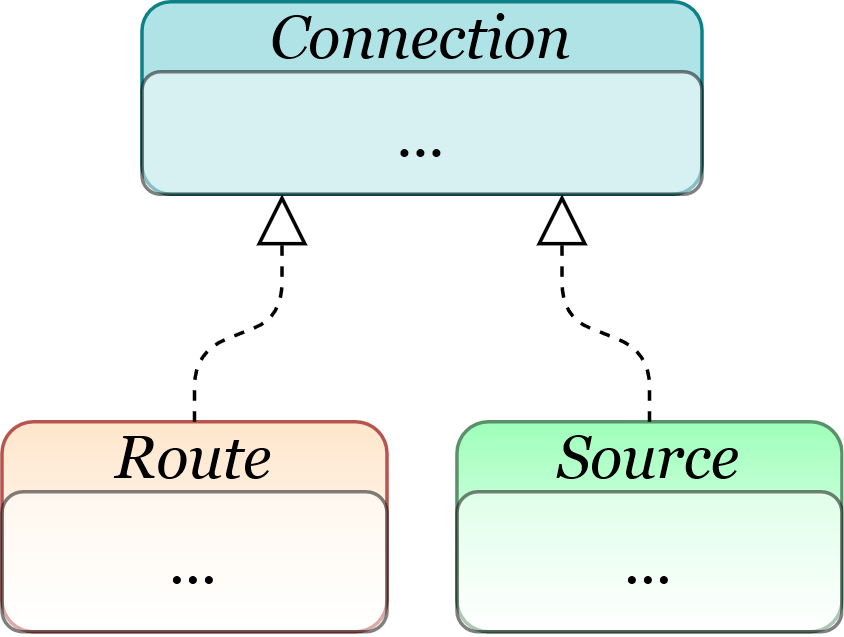
\includegraphics[width=0.35\textwidth]{PICs/NARU/naru-connection-types.png}
    \caption{Connection Types}
    \label{connection-types}
\end{wrapfigure}

 
The connections between bundles will be segregated into two distinct categories, which will be referred to as \textbf{routes} and \textbf{sources}.   
If a bundle \textbf{A} is connected to a bundle \textbf{B} and this connection is of type 
\textbf{route} then the connection of \textbf{B} to \textbf{A} will be of type \textbf{source}. 

Both connection types are identical in terms of their computation graph, however
they differ in terms of their purpose.
Although information can flow from \textbf{A}
to \textbf{B}, conceptually only the source connection will be treated as the intended direction for the flow of information.
 

This relationship between two bundles, as illustrated by the Figure \ref{connecting-naru-bundles} below, still lacks the core attribute which distinctly defines conditional neural networks, namely: \textbf{sparse activity}. \linebreak
To achieve this within a network of connected bundles we only want to activate a subset of bundles (and their connections) for a given time step. The responsibility of choosing which bundle ought to be activated next will be placed on a currently active bundle which can select a connected bundle based on a simple routing algorithm which utilizes the \textbf{route} type of connection between the two bundles.
 

\begin{figure}[h]
    \centering 
     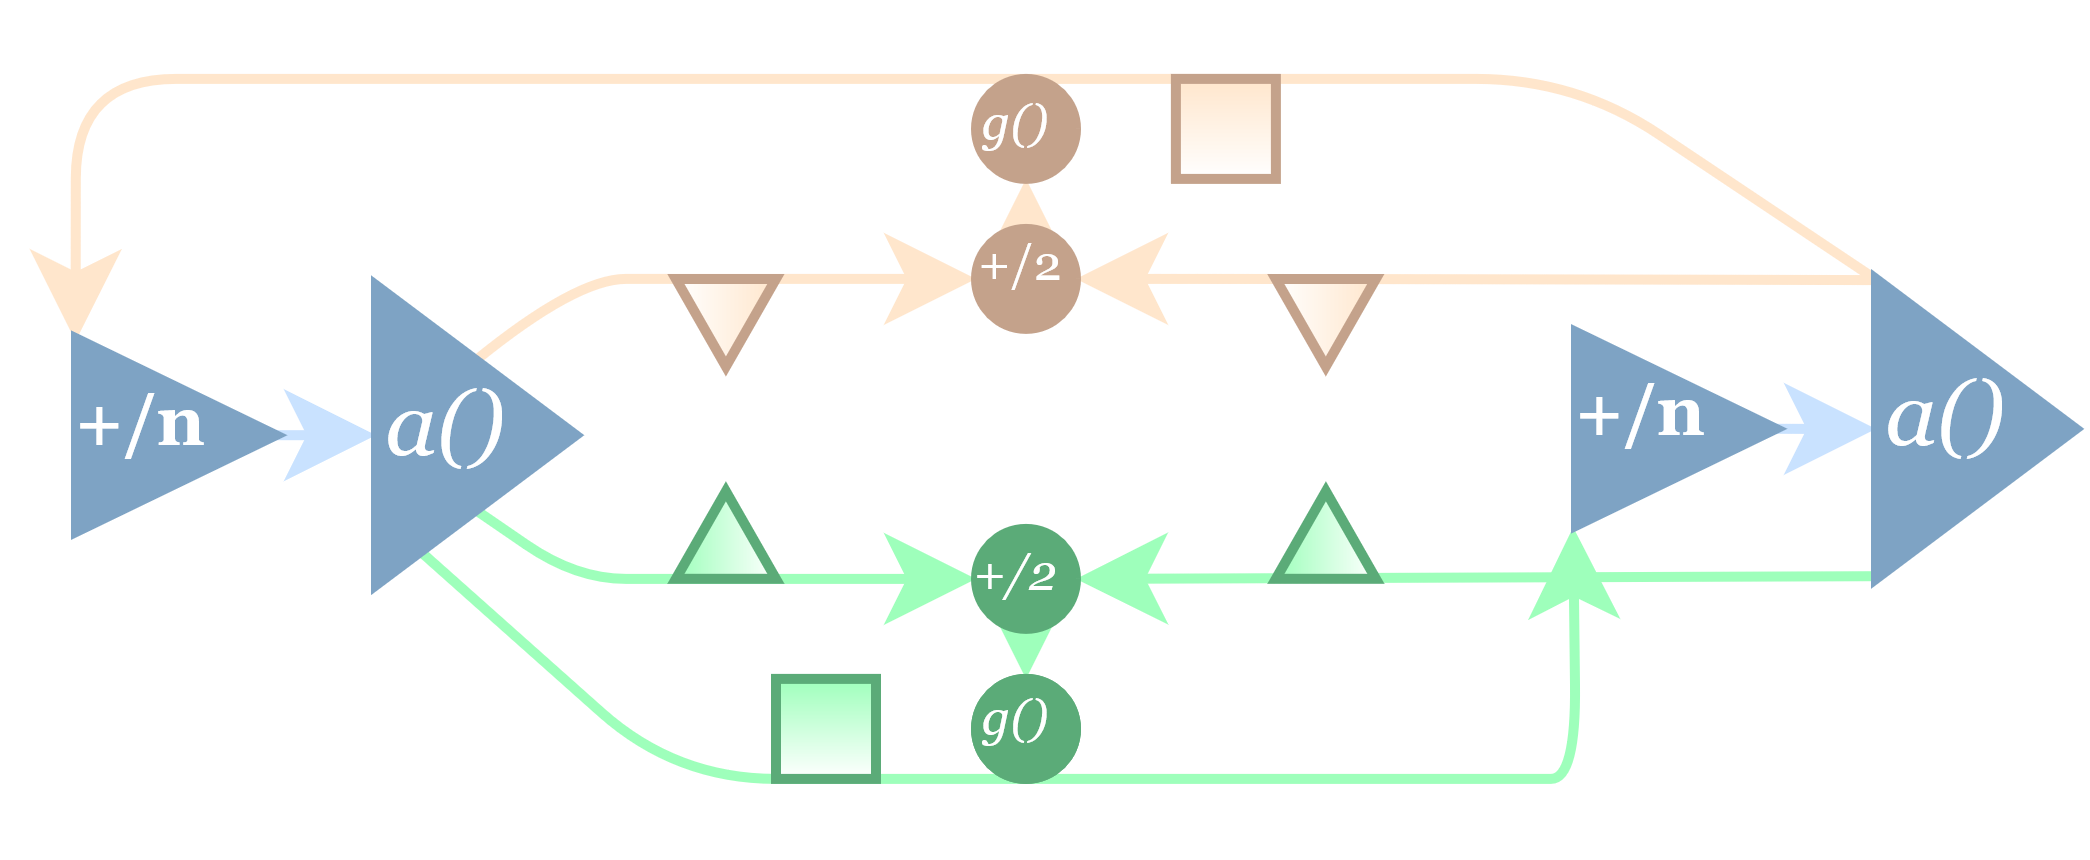
\includegraphics[width=\textwidth]{PICs/NARU/connected-naru-bundles.png}
    \caption{Two Interconnected Bundles}
    \label{connecting-naru-bundles}
\end{figure}


So for a given bundle \textbf{A}, having route connections to other bundles \textbf{B}, \textbf{C} and \textbf{D}, the routing algorithm will determine which one of \textbf{B}, \textbf{C} and \textbf{D} ought to be activated next based on the corresponding gating mechanism of the route connections to \textbf{B}, \textbf{C} and \textbf{D}.
 
 \clearpage
%----------------------------------------------------------------------------------------------

As previously established, connections are in essence gated inputs for their respective bundles.
Conceptually one could assume that the gate value produced by the gating function of a given connection serves as a score for the importance of the bundle state to which it connects. This role would simply emerge during training, because the gating mechanism would converge to a state in which it acts as an attention mechanism allowing bundles to selectively observe other bundles. \linebreak
 
 If a current bundle deems another one as important
then this assumption also infers that the information encoded in this other bundle is useful, meaning that \textbf{both bundles might share very similar responsibilities}.  
In that case it is reasonable to assume that the other bundle could be activated next.
This reasoning leads to the following conditional routing algorithm:\linebreak
 

\begin{quote}
\textbf{\textit{For a given currently active bundle, the bundle which ought to be activated next will be chosen by the route whose gate value is the largest among all the route connections of the current bundle. }}
\end{quote}

\begin{figure}[h]
    \centering 
     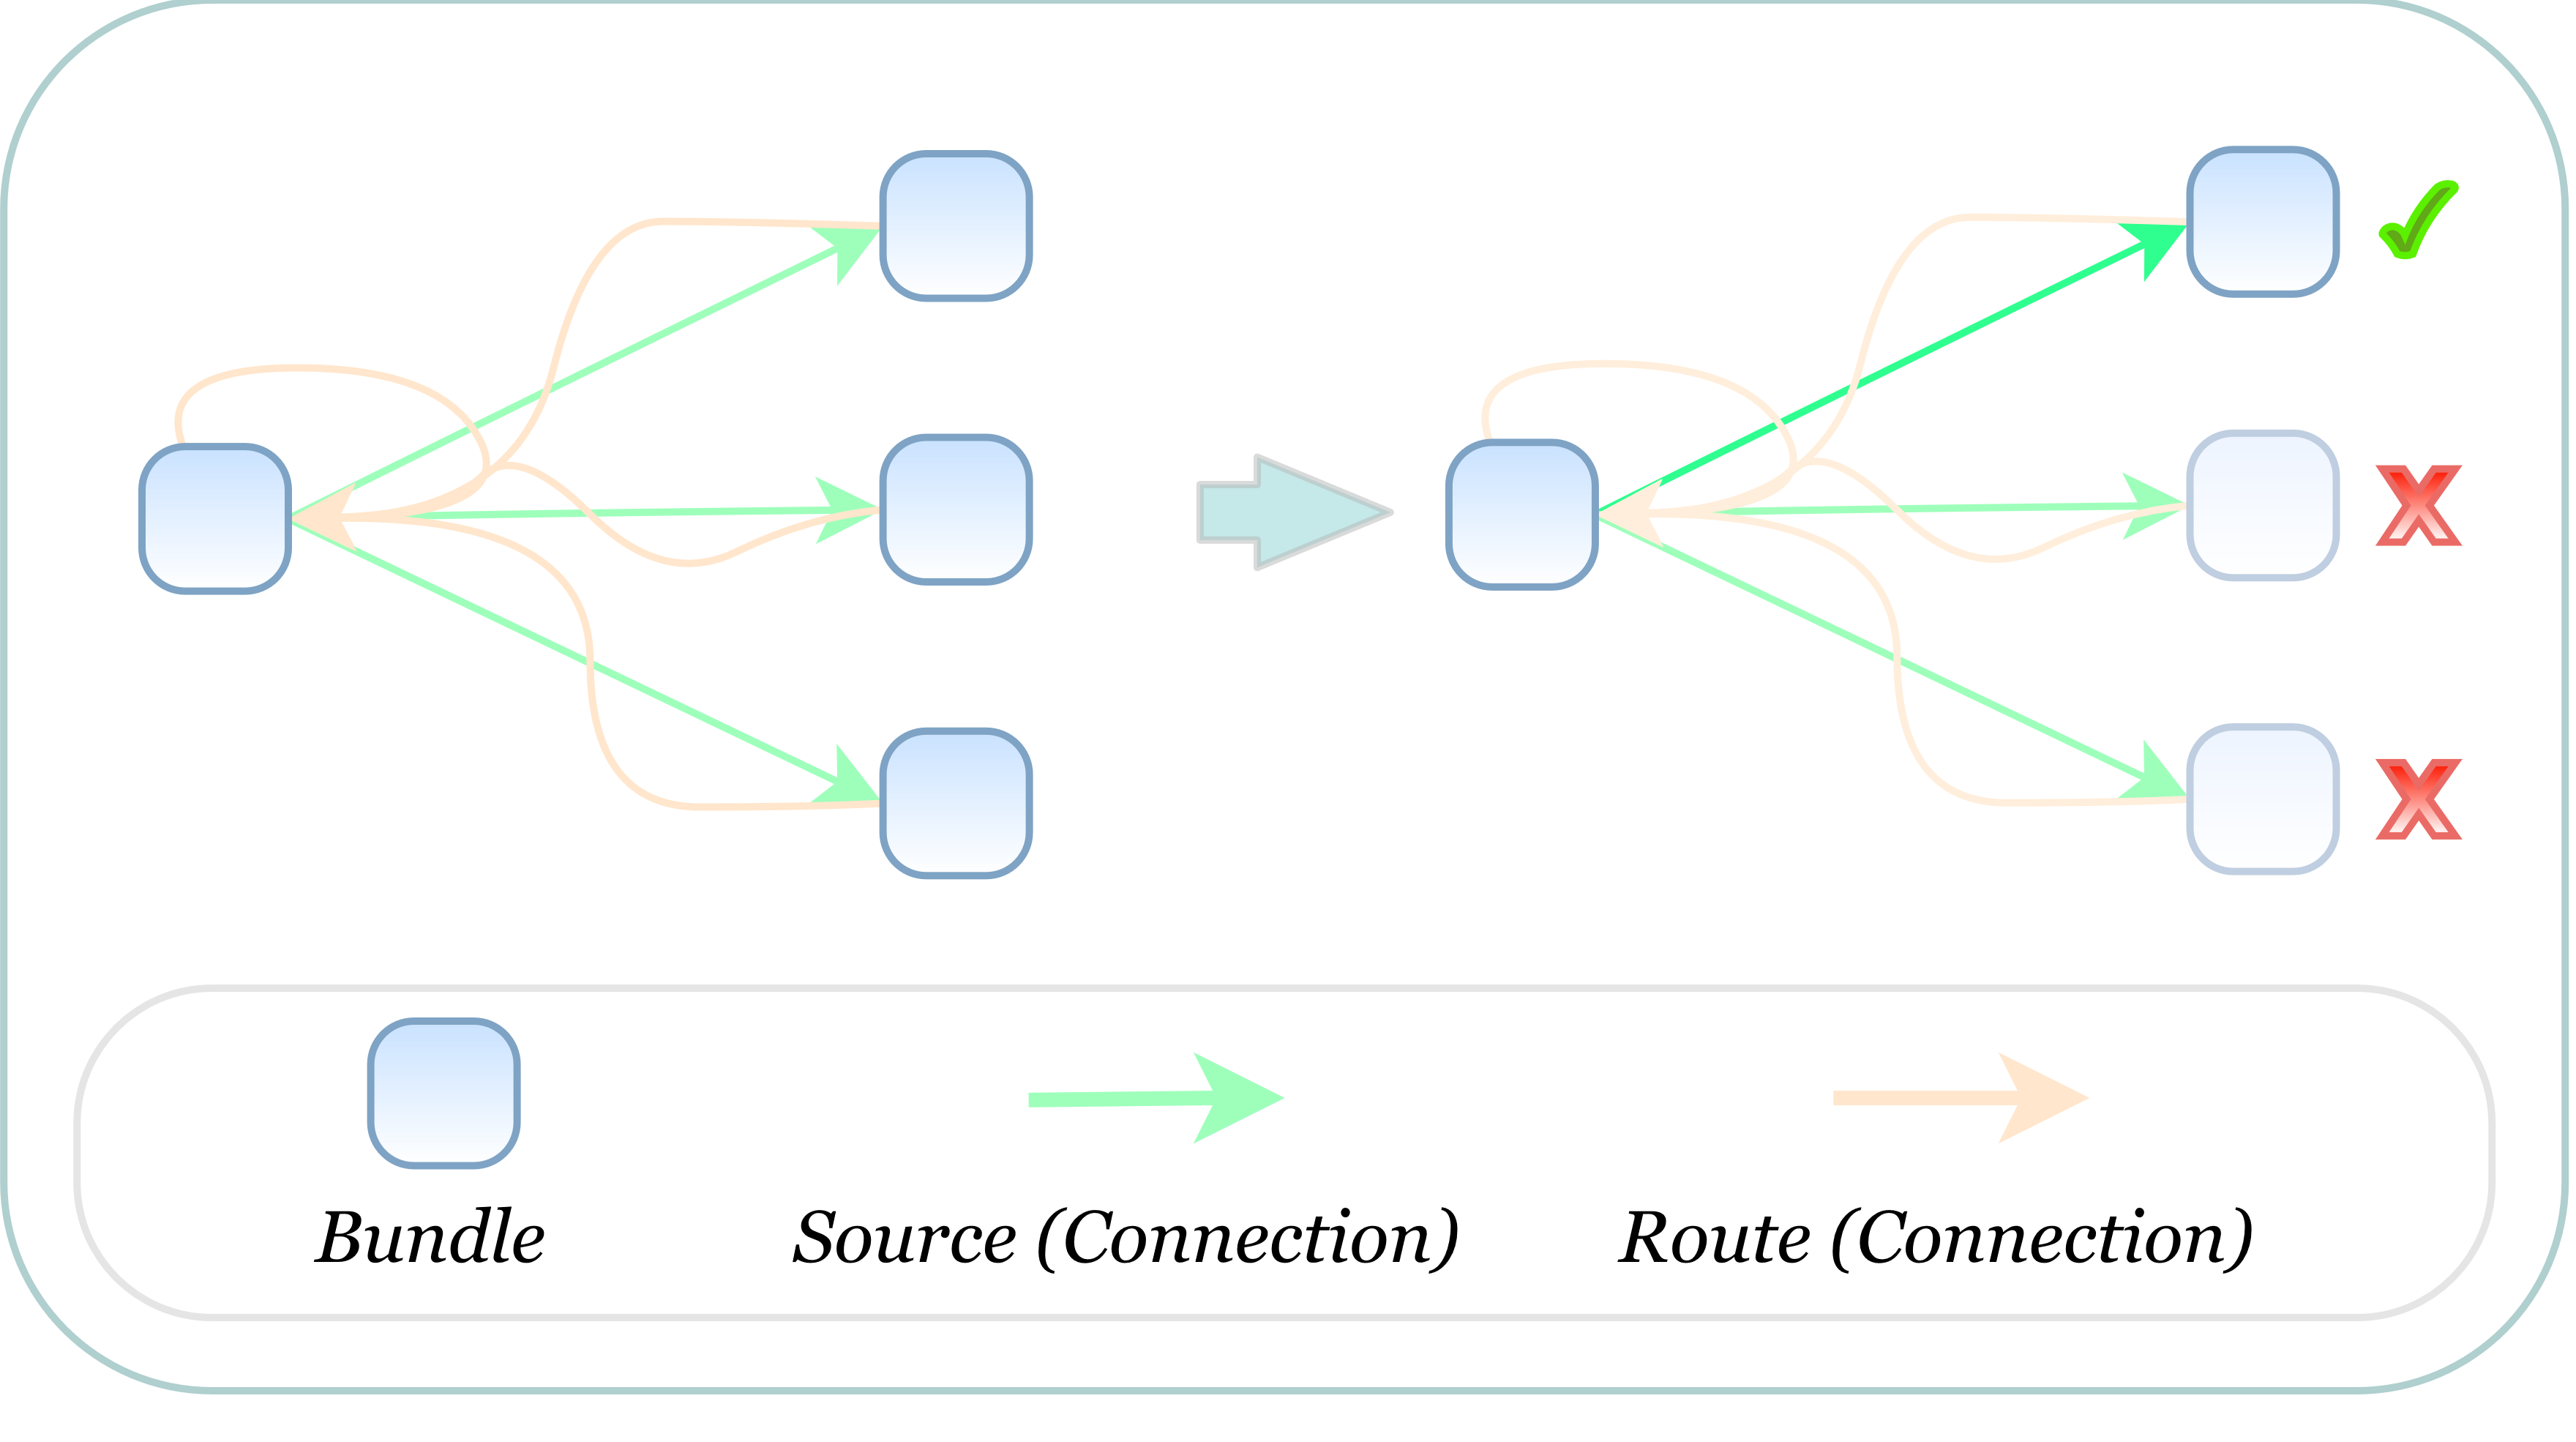
\includegraphics[width=\textwidth]{PICs/NARU/directed-routing.png}
    \caption{Directed Routing between interconnected Bundles}
    \label{directed-routing-illustration}
\end{figure}

When constructing a network of \acp{NARU}, the previously defined distinction between routes and sources allows for a directed flow of information
throughout the entire network. As illustrated by the \acs{NARU} in Figure \ref{directed-routing-illustration},
the single bundle connected to 3 other bundles can choose which
one of them ought to be active next, however these bundles cannot 
elect the left bundle.

\clearpage
%----------------------------------------------------------------------------------------------


\section{Avoiding Routing Bias}

As discussed in subsection \ref{subsec_routing-bias}, a major challenge of
\acp{CDLN} is routing bias, the phenomenon that the routing mechanism
does not choose the network sub-sets evenly.
In order to prevent the emergence of this bias during training,
\acs{NARU} was purposefully designed without the use of a bias
as additive parameter to the pre-image of non-linear activation 
functions.  \\
As can be observed in equation \ref{eq_bundle-activation}, the activation 
for a given bundle does not involve the use of an additional vector of parameters.

\begin{gather} 
\mbox{\LARGE$\displaystyle
 a( \frac{\sum_{i=1}^{n} c_i}{n} \cancel{ + b} )  
$}
\end{gather}

This design choice is based on the reasoning that the input to a given bundle
will consist of a set of connection output vectors which has previously been active
and another set of vectors which has been inactive.
Because among all connections of a given bundle only a single connection will be 
elected as route, the majority of bundles will be constant.
Consequently the states of the majority of connection outputs will simply
vary based on the gating scalar between 0 and 1, as is defined by equation \ref{eq_gate}, however the encoded information
would only be lost to that degree.


\begin{gather} 
\mbox{\LARGE$\displaystyle
 a( \frac{\sum_{i=1}^{n} c_i}{n} ) 
 \longrightarrow 
 a( \frac{\sum_{i=1}^{|A|} c_{a_i}}{|A|} + \frac{\sum_{i=1}^{|B|} c_{b_i}}{|B|}  ) 
$}
\end{gather}

When segregating this conceptual group of active input vectors into set \textit{\textbf{A}}
and the set of relatively constant input vectors into set \textit{\textbf{B}}, then
this resembles the usage of a bias. 
However, contrary to the traditional bias, this virtual bias is not constant because it is
dependent on the states of a potentially larger number
of dormant \acp{NARU} whose states can mutate over longer periods of time. \\

This makes the state of this virtual bias dependent on the inputs fed into the network. \\
If a given model receives information for which it has not been trained, then
this would consequently lead to noise in the gating mechanism which also leads to a more random decision made by the routing algorithm as is defined in section \ref{sec_naru-routing}. The routing should therefore be more unbiased when encountering unexpected information.  

\clearpage
%----------------------------------------------------------------------------------------------

\section{Directed NARU Networks}

The concrete architecture tested in this thesis
is a composition of \acp{NARU} forming a graph in
which activity is being routed directly towards the end of the network.
However the activation paths will always have
the same length, which is equals to the depth of the network.
Conversely, allowing activity to be routed in cycles
would cause the execution time and cost of a single forward pass
to be fluctuating and most likely also to be unpredictable.

Due to the gating mechanism of a single unit, this architecture is conceptually a \acl{RNN} in which information can flow in cycles. 
This is evident by equation \ref{eq_full-connection-feed-forward} as well
as the routing mechanism which consists of connections directed towards the flow
of information within a network of \acp{NARU}.

\begin{figure}[h]
    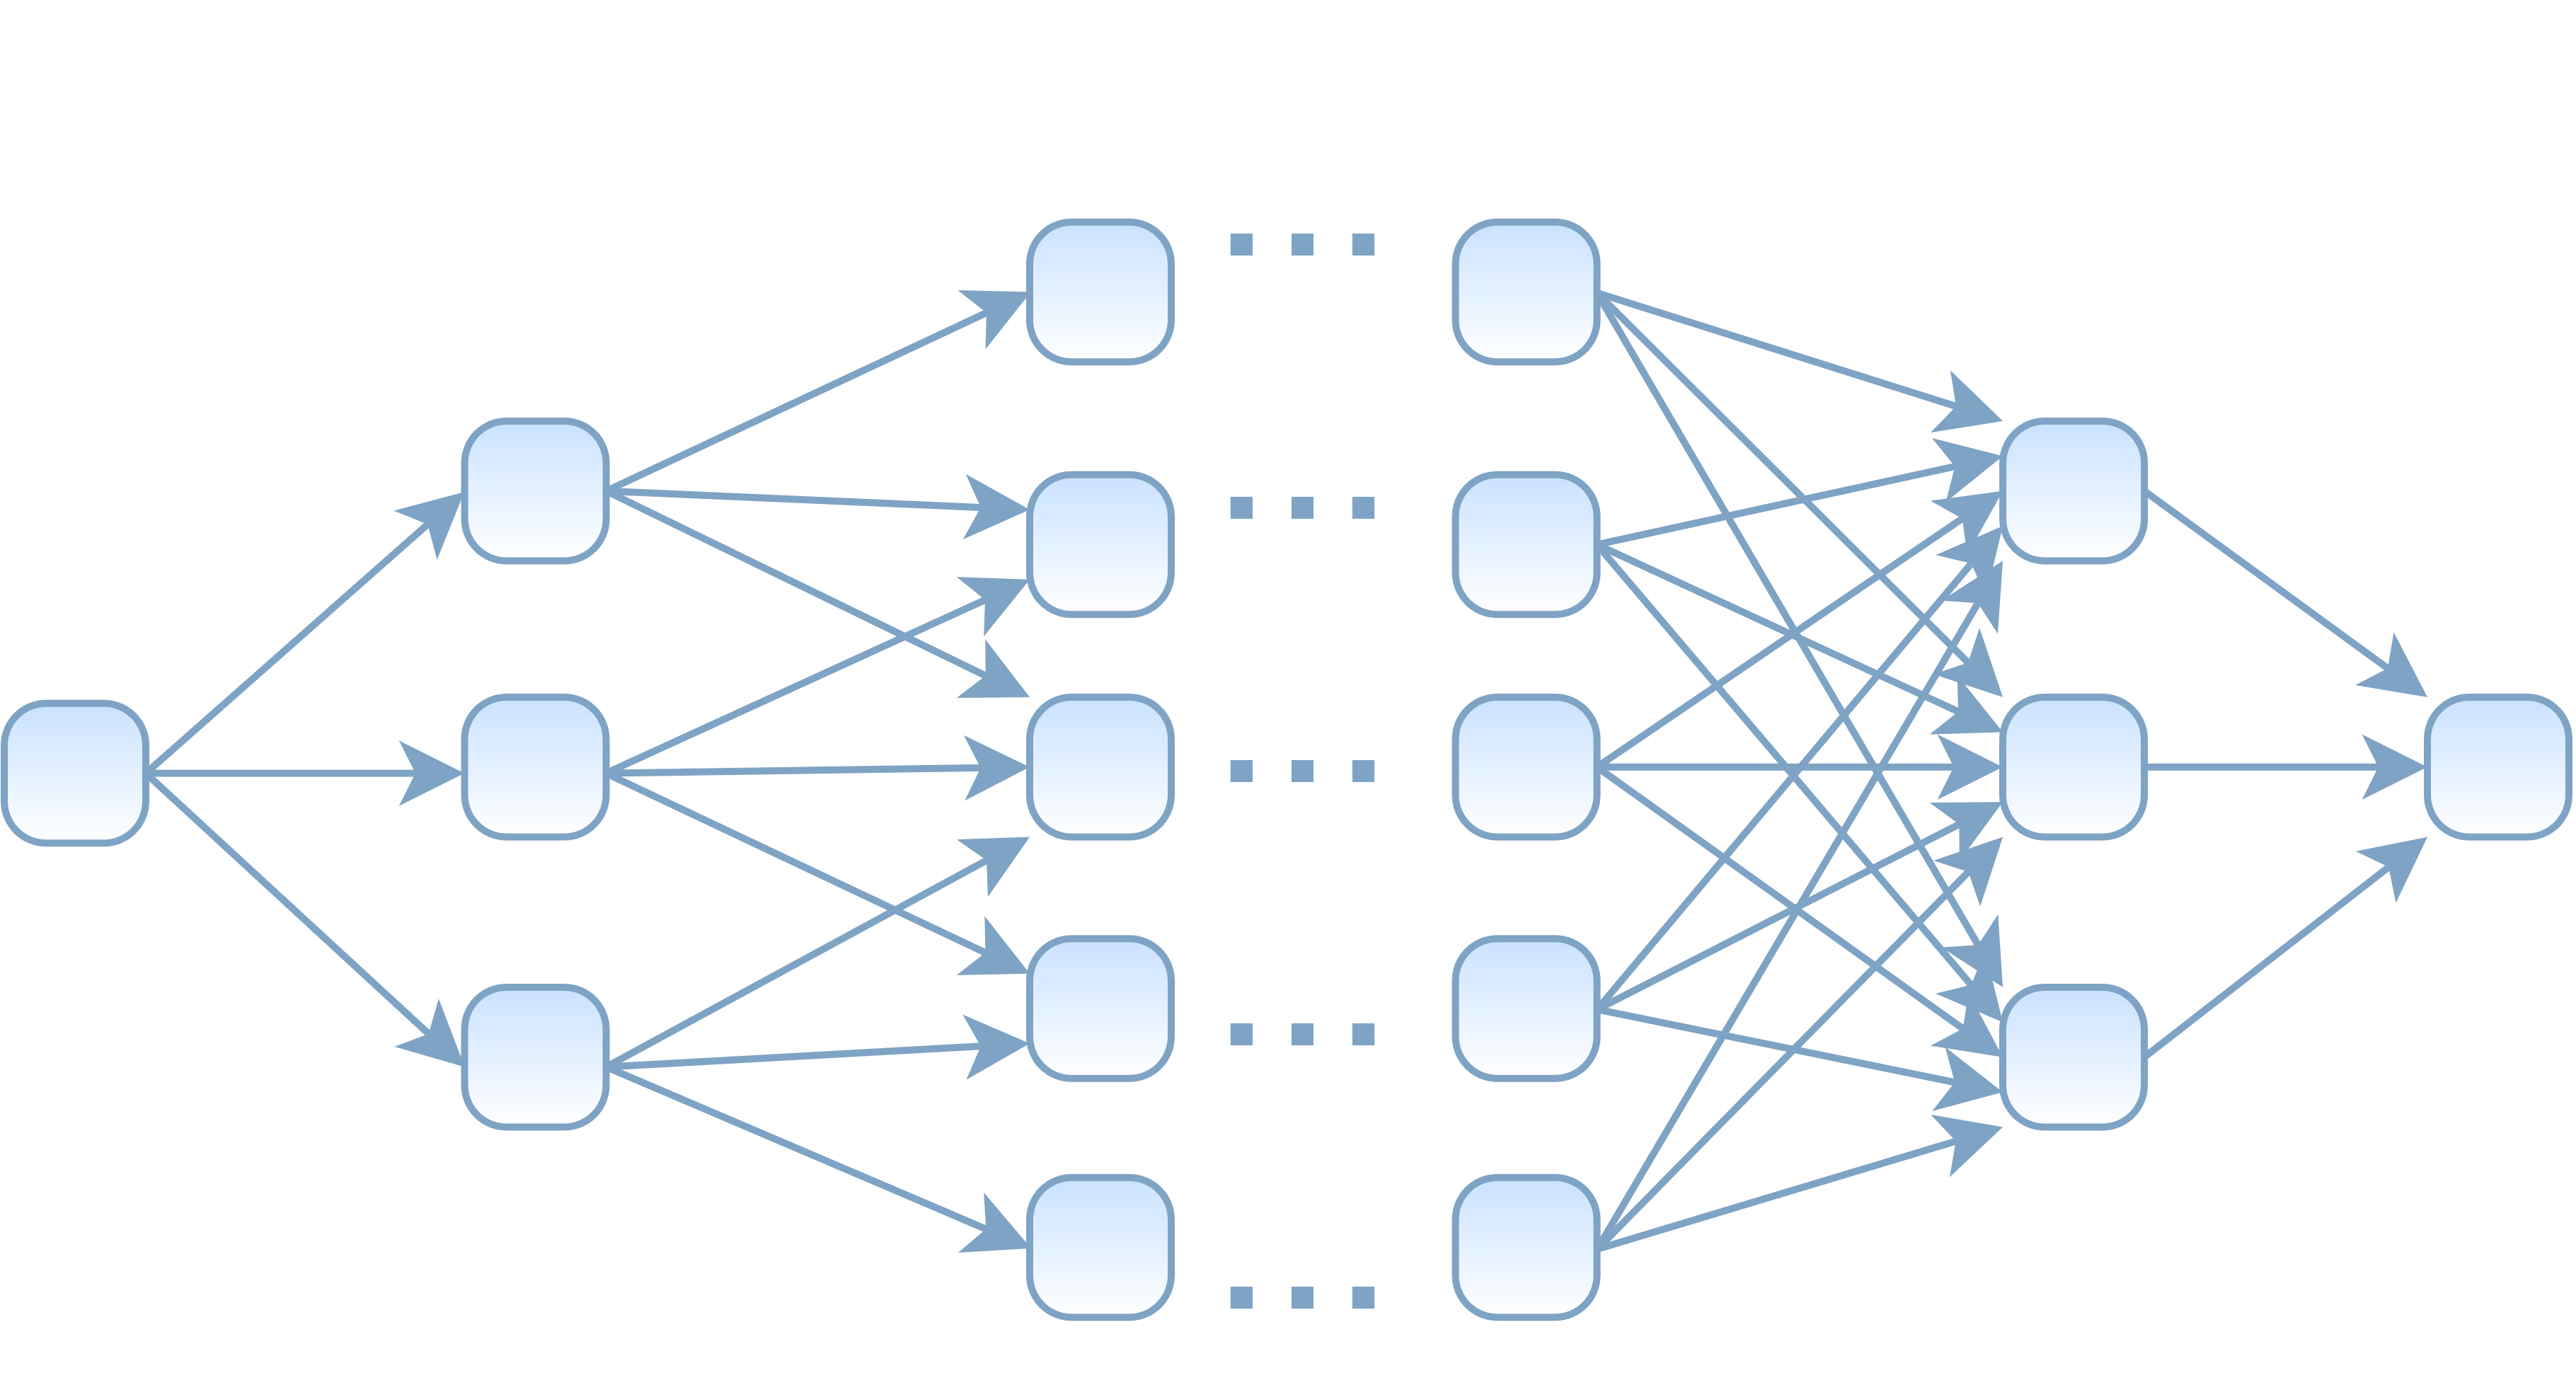
\includegraphics[width=\textwidth]{PICs/NARU/directed-naru-net.png}
    
    \caption{A Directed Network of NARUs}
    \label{naru-net}
\end{figure}

The vertically stacked bundles illustrated in
Figure \ref{naru-net} will be referred to 
as \textit{capsules} similar as in the stacked layers described in  "\citetitle{15_dynamic-routing-between-capsules_2017}" \cite{15_dynamic-routing-between-capsules_2017}.
Every bundle within a capsule will be structurally
identical, however bundles not within the same
capsule might have different input and output dimensions.\linebreak
The degree of interconnectedness between capsules
will be limited by a \textit{maximum cone size}.
A single bundle cannot have more
connections than this threshold.
The reason for this sparsity is to save 
computational cost. The cone size
does not need to be larger than the 
size growth (number of bundles) between two consecutive capsules in order to
make it possible for an input signal 
to be able to visit any bundle in the entire network.

\clearpage
%----------------------------------------------------------------------------------------------

\subsection{Model Specification}\label{subsec_model-specification}
      
The model consists of a total of \textit{7 capsules}, each of which contains
a number of bundles ranging \textit{from 1 to 18}.
These capsules are connected with a \textit{maximum cone size of 6}.


\begin{table}[h] 
\centering
 \begin{tabular}{||c || c c c c c c c ||} 
 \hline
   Capsule & 1 & 2 & 3 & 4 & 5 & 6 & 7 \\ [0.5ex] 
 \hline\hline
 Number of bundles & 1 & 6 & 12 & 18 & 12 & 6 & 1  \\ 
 \hline
 Bundle dimensions & 50 & 76 & 102 & 128 & 102 & 76 & 50  \\ 
 \hline
 Routes per bundle & 6 & 6 & 6 & 6 & 6 & 1 & 0 \\
 \hline
 Sources per bundle & 0 & 1 & 3 & 4 & 9 & 12 & 6 \\  
 \hline
\end{tabular}
\caption{Structural Summary of the Tested Model}   
\end{table}  

This model receives inputs in the form of tokens encoded into
vectors matching the input dimensionality of 50. \\

This embedding has been based on the technique outlined in \cite{web_embedding-howto}.
The embedding used for this experiment was \cite{web_embedding-glove},
a pre-trained mapping between a total of 400 thousand tokens 
alongside corresponding vectors of size 50.

\clearpage
%----------------------------------------------------------------------------------------------


\begin{figure}[h]
\centering
    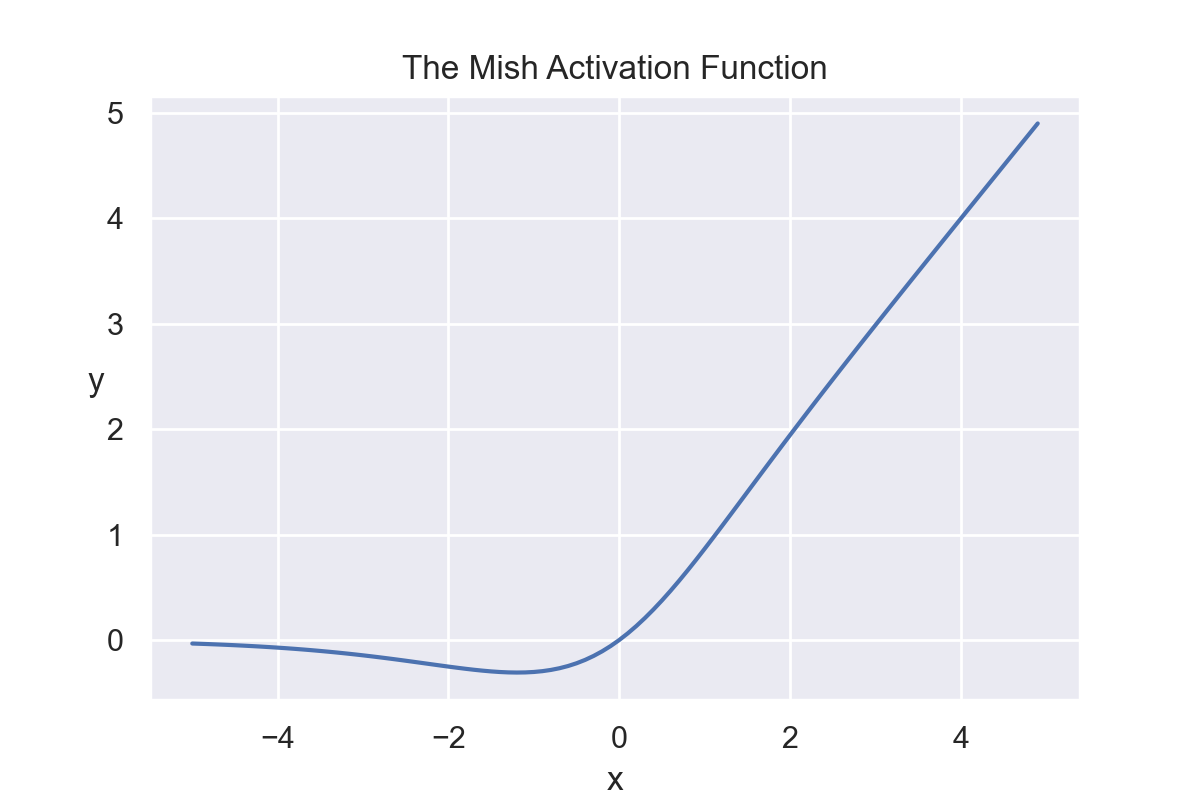
\includegraphics[width=\textwidth*2/3]{PICs/Results/mish-activation.png}
    
    \caption{The used activation function \textit{\textbf{a()}}}
    \label{mish-function}
\end{figure}

The activation function used for the implementation of \textit{\textbf{a()}}, as is defined
in equation \ref{eq_bundle-activation}, is the so called \textit{Mish activation function}, which is defined as:

\begin{alignat}{1}\label{eq_mish}
 f(x) = x * tanh(softplus(x)) 
\end{alignat}

The usage of this function is based on the findings reported in \citetitle{32_mish-misra2020} \cite{32_mish-misra2020}, which show improved convergence for very deep models with a large number layers. Although the model tested in this thesis does not have many layers, it still propagates information recurrently through time. \\

The source code for the implementation of this concrete model specification alongside the test setup can be viewed at \cite{naru-github}.
 
 \clearpage
%----------------------------------------------------------------------------------------------
 
\section{Results}

The model specified in subsection \ref{subsec_model-specification}
was trained across \textit{200 epochs}
using a data set containing \textit{1500 sentences
with an average length of 25 tokens}.
Due to the high degree of branching
of this architecture, the use of batches
in the form of single tensors containing multiple
samples was not possible.
Instead \textit{small batches containing 10 sample}
were fed into the network sequentially, for every epoch. After which the accumulated gradients were divided by the batch size to form an average gradient which was then applied to the
weights. 


\begin{figure}[h]
    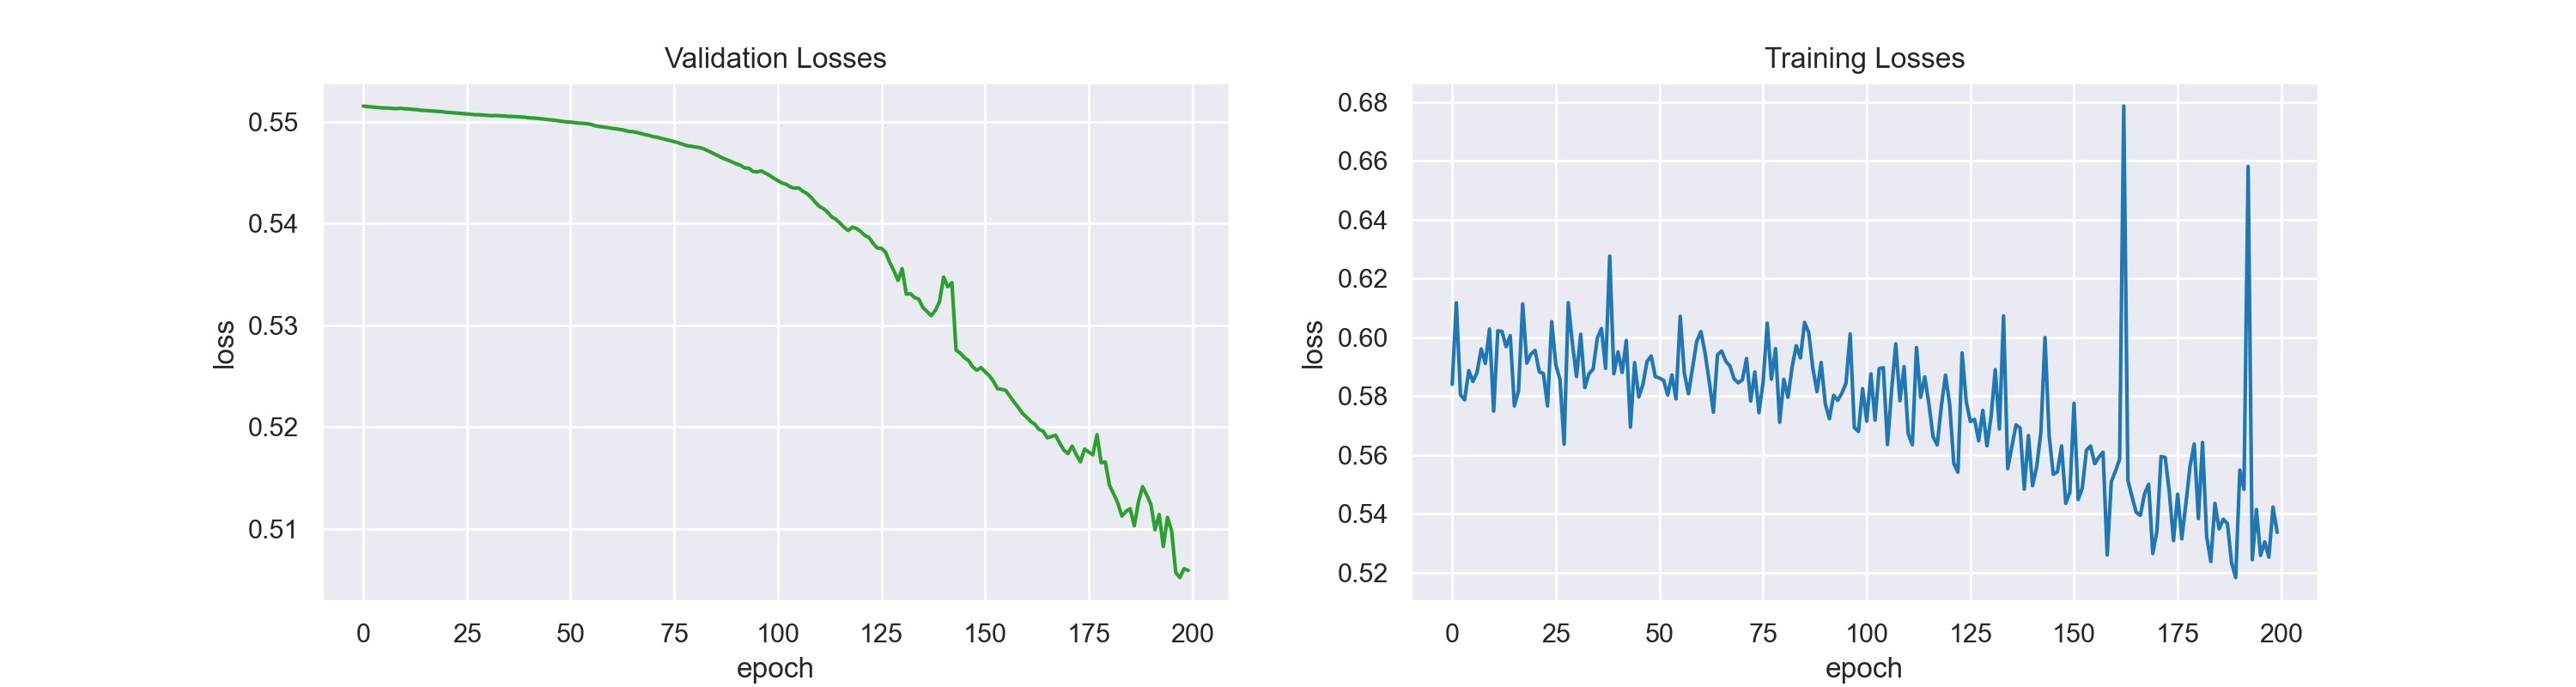
\includegraphics[width=\textwidth]{PICs/Results/validation-and-training-loss.png}
    
    \caption{Validation and Training loss for a directed NARU network}
    \label{results-validation-and-training}
\end{figure}

As can be observed in Figure \ref{results-validation-and-training},
the model converged reliably and the validation
loss also decreased throughout the 200 epochs.
However the rate of convergence was very slow
and noisy. 
Due to the high degree of branching
the use of accelerator hardware did not yield
a speed-up in training time. Therefore longer training sessions were not feasible 
as the already performed training was incredibly time
consuming. 


\clearpage
%----------------------------------------------------------------------------------------------

The routing behavior of the network has been measured
throughout the training session by recording
the indices of the active bundles for every
capsule within the network.
This information has been used to raise
a variety of metrics, namely
\textit{activity saturation}, 
\textit{route reorganisation} and
\textit{routing bias}.
These metrics will be displayed and discussed for further examination in the following paragraphs.\linebreak

In order to validate the claim that the network 
would only use a subset of parameters to perform
a prediction, the degree of \textit{cumulative total 
network utilisation} was raised from the taken measurements for every sentence in every epoch.

\begin{wrapfigure}{L}{0.60\textwidth}
  \centering 
  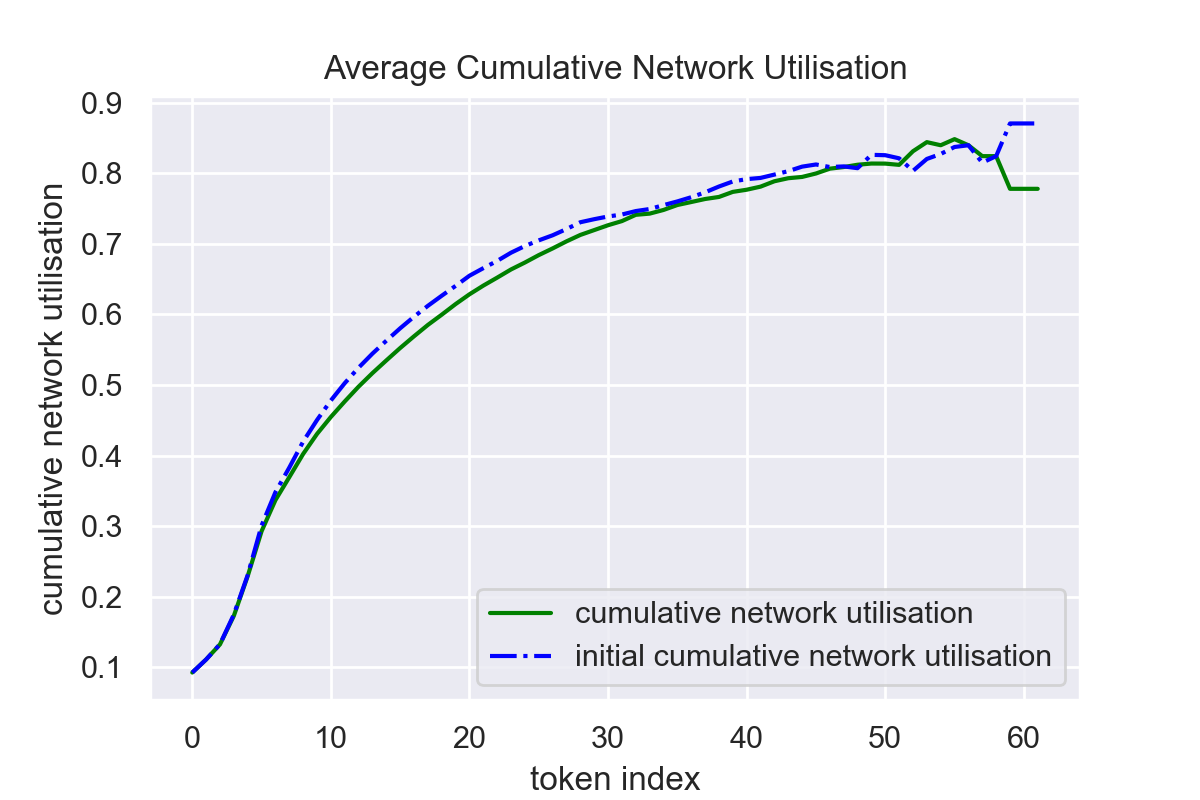
\includegraphics[width=0.60\textwidth]{PICs/Results/cumulative-network-utilisation.png}
  \caption{The Cumulative Network Utilisation}
  \label{results-network-utilisation}
\end{wrapfigure}


Figure \ref{results-network-utilisation} shows
the average network utilisation across all epochs.
The x axis represents both the token index of a given sentence as well as the time step.

Besides to total average across all epochs,
Figure \ref{results-network-utilisation} also displays
the initial cumulative activity saturation of the 
network in order to indicate how this metric 
has changed during training.

The rate of saturation slightly decreased over time
which might indicate that the architecture has learned
to use its bundles selectively to 
predict tokens within a given sentence.
 
\clearpage
%----------------------------------------------------------------------------------------------

\begin{wrapfigure}{R}{0.60\textwidth}
  \centering 
  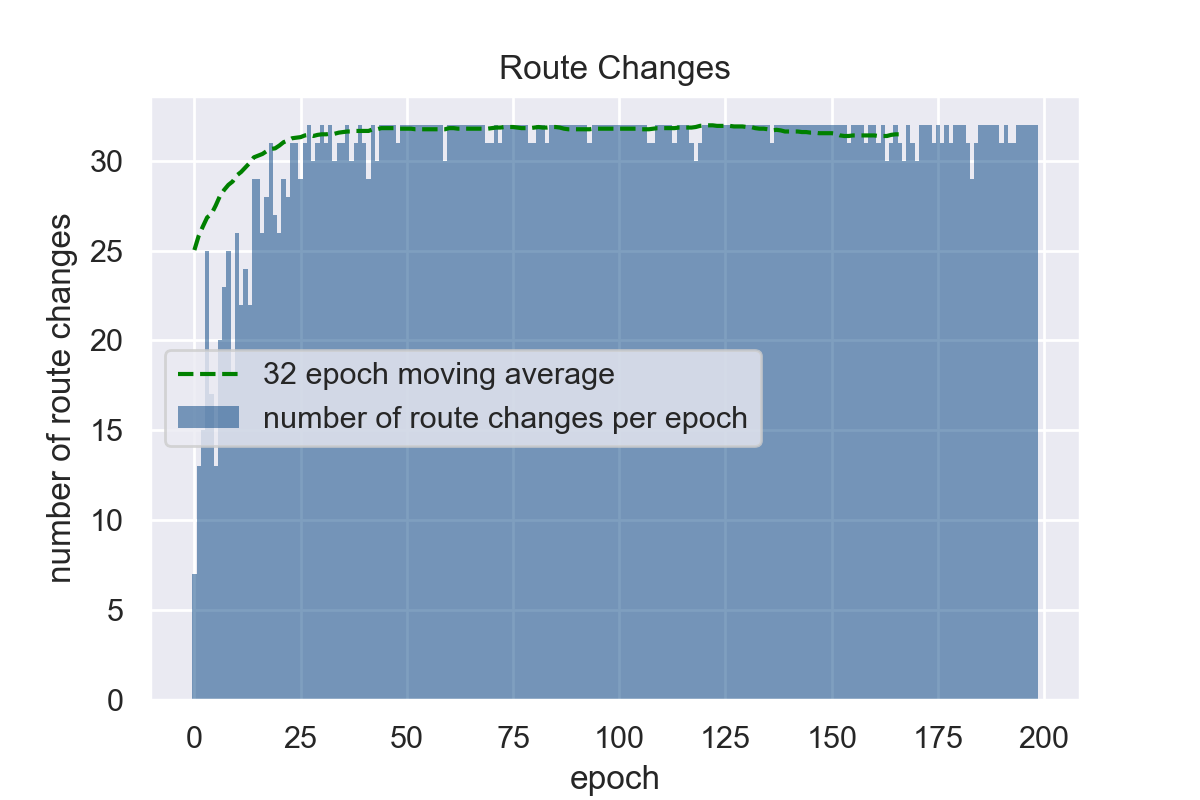
\includegraphics[width=0.60\textwidth]{PICs/Results/route-changes.png}
  \caption{Frequency of route changes during training}
  \label{results-route-changes}
\end{wrapfigure}
 
  

Figure \ref{results-route-changes} shows the number
of route changes across all sentences for every epoch.
Route changes were measured for every sentence within the training data. A route change is always based on a recording of the previous route generated by a given sentence.
Conceptually, this metric can also be understood
as a degree of internal reconfiguration.
If the weights are not updated then no changes will
occur when a sentence is reintroduced to the network.
This is simply because it will deterministically produce the exact same predictions as previously.
This might change however upon updating the weights of the network.
Because this metric contains high levels of noise
an additional moving average was introduced
which ought to enable the ability to identify a 
potential trend.\break

As has already been discussed in subsection \ref{subsec_routing-bias}, a major
challenge of \acs{CDLN} has been the emergence of routing
bias during training. 

\begin{wrapfigure}{L}{0.60\textwidth}
  \centering 
  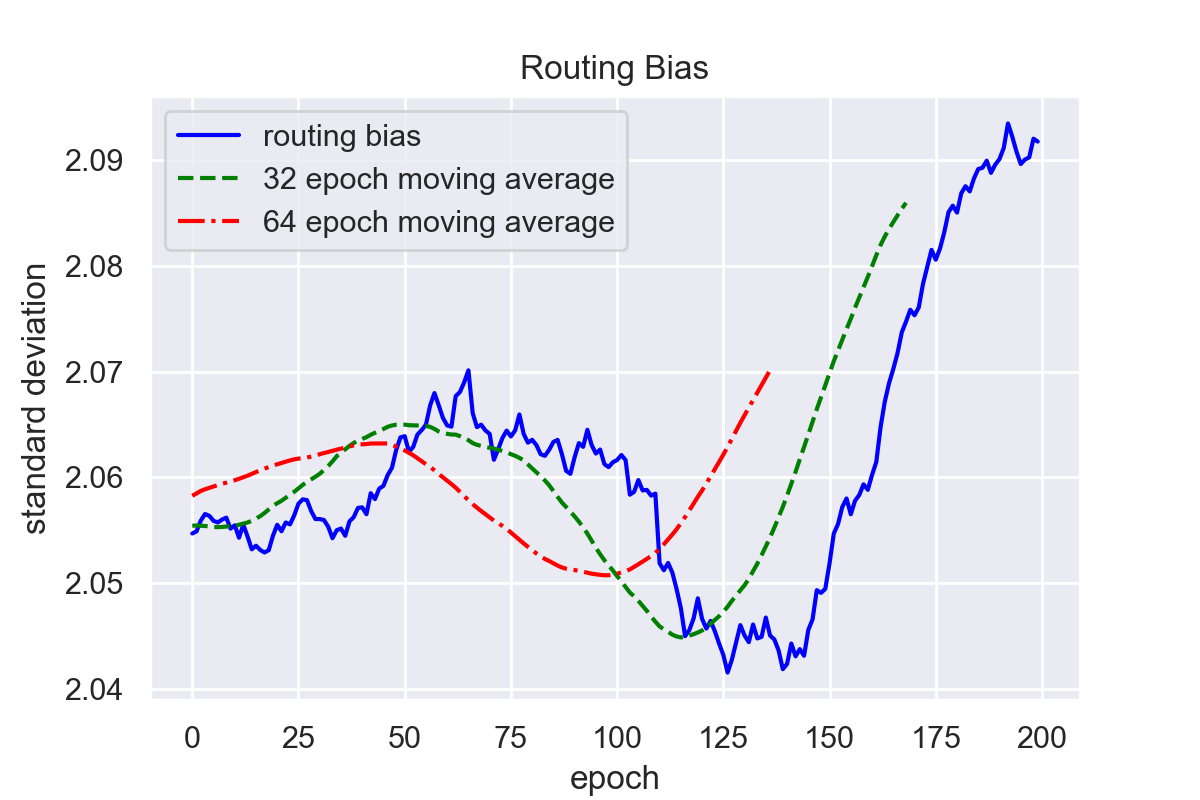
\includegraphics[width=0.60\textwidth]{PICs/Results/routing-bias.png}
  \caption{Change in Routing Bias during Training \break (accumulated deviation from expected average)}
  \label{results-routing-bias}
\end{wrapfigure}


In order to detect the emergence of said bias, the standard deviation
of the distribution of routes was calculated for all epochs during training.
This metric can be observed in Figure \ref{results-routing-bias}, which shows
how the standard deviation changes throughout the entire training session.

Two additional moving averages were introduced
in order to help identifying potential trends.
However there seems to be no statistically significant 
trend which might indicate that a routing bias exists or would ever emerge.


\clearpage
%----------------------------------------------------------------------------------------------


\chapter{Conclusion}
Based on the categorization of \acs{ANN} architectures 
established in section \ref{sec_common-properties} chapter \ref{chap_state-of-the-art}, we suggest that 
many design approaches for state of the art \acs{ANN} architectures
are very dissimilar to \acp{BNN} in potentially unfavorable ways.
The most relevant of which would be sparsity, which means that large parts of a neural network stay either inactive for a given period of time, or fire in a less frequent manner.
This property observable in \acp{BNN} allows them to utilize neurons selectively.
It has been theorized that this is due to reasons related to energy efficiency as well as memory locality, where neurons encode information that might not be needed for longer periods of time \cite{7_dorment-brain_2015}. 
A novel type of architecture tries to overcome these challenges at least partially.
So called “Conditional Neural Networks” or “Conditional Deep Learning Networks” have been successfully trained to route information based on various gating/routing mechanisms, improving both energy efficiency as well as accuracy compared to state of the art architectures \cite{8_CDL-4-efficient_2015}\cite{11_efficient-CDL_2017}\cite{12_dynamic-routing-in-ANNs_2017}.
These types of networks have also yielded promising results for
transfer and online learning \cite{31_continual-learning-2020} as well as reinforcement learning \cite{27_path-net-evolution}. 
However this approach also faces major challenges, namely the emergence of routing bias and the difficulty of applying batches during training. 


 
 